%%%%%%%%%%%%%%%%%%%% author.tex %%%%%%%%%%%%%%%%%%%%%%%%%%%%%%%%%
%
% Template de Springer Nature (SNmult) limpio para proyecto de investigación
%
%%%%%%%%%%%%%%%% Springer Nature %%%%%%%%%%%%%%%%%%%%%%%%%%%%%%%%

\documentclass[graybox]{SNmult}

% PAQUETES DE FUENTE Y FORMATO RECOMENDADOS POR SPRINGER
\usepackage{type1cm}
\usepackage{makeidx}
\usepackage{graphicx}
\usepackage{multicol}
\usepackage[bottom]{footmisc}

\usepackage{newtxtext}
\usepackage[varvw]{newtxmath}

\usepackage{tikz}
\usetikzlibrary{automata, positioning, arrows.meta}

\makeindex

\begin{document}
	
	\title*{Análisis Estocástico de la Evolución de Patologías y Evaluación del Impacto Farmacológico mediante Procesos de Galton-Watson}
	\titlerunning{Simulación Estocástica de Patologías} 
	
	\author{Sofía Rodríguez Peláez}
	
	\institute{Sofía Rodríguez Peláez \at Grado en Ingeniería Informática y Grado en Estadística, Universidad de Valladolid, \email{sofia.rodriguez23@estudiantes.uva.es}}
	
	\maketitle
	
	% ABSTRACT PARA PUBLICACIÓN ONLINE
	\abstract{Este trabajo analiza la evolución estocástica y la dinámica de transmisión de una patología en una población finita mediante un Proceso de Ramificación de Galton-Watson. El modelo incorpora mortalidad prematura basal ($m_0=0.05$), severidad patológica ($m_1=0.60$) y probabilidades condicionales de transmisión por herencia ($p_1=0.95$) y mutación ($p_0=0.15$). Debido a la naturaleza estocástica del sistema se justifica e implementa una simulación Monte Carlo con $M=500$ réplicas independientes para caracterizar el comportamiento esperado de la población para tratar de eliminar esa aleatoriedad. Se evalúa la convergencia hacia el estado absorbente de extinción total ($N=0$), estimando la esperanza matemática del tamaño poblacional $\mathbb{E}[N_t]$ junto con su intervalo de confianza al 95\%. Los resultados confirman la no supervivencia de la población en el caso base sin intervención, alcanzando una probabilidad de extinción del $100\%$ ($\eta=1.0$) y determinando un tiempo medio hasta la absorción de $\mathbb{E}[T_{\text{abs}}] \approx 72$ generaciones. Posteriormente se estudia el impacto de diferentes fármacos como alternativas a la enfermedad y se obtienen conclusiones sobre los resultados de supervivencia y extinción en la población.
		\keywords{Procesos de Ramificación $\cdot$ Galton-Watson $\cdot$ Simulaciones Monte Carlo $\cdot$ Estado Absorbente $\cdot$ Dinámica Poblacional}}
	

	
	\section{Introducción}
	\label{sec:introduccion}
	En este apartado se pretende contextualizar sobre el problema biológico y genético del problema, explicar por qué se decide estudiar de esta forma y las ventajas que puede presentar y, por último, explicar el caso base y las diferentes estrategias farmacológicas que se han decidido utilizar para solucionar el problema. 
	Se parte de una población mayoritariamente sana que tiene una cierta proporción significativamente menor de individuos enfermos. 
	\subsection{Contexto biológico y genético del problema}
	Primeramente es importante destacar que este problema es hipotético, no está basado en ningún caso real documentado. El problema podría existir en la realidad, pero en este caso los parámetros como las probabilidades de herencia y de fallecimiento han sido elegidos de manera aproximadamente aleatoria, jugando con los parámetros para obtener un modelo interesante que pueda erradicar la población para, posteriormente, permitir estudiar diferentes estrategias que permitan la supervivencia de la población. 
	
	Se parte de una población mayoritariamente sana con una cierta proporción de individuos que presentan una mutación genética que provoca una enfermedad. En algunas ocasiones, esta enfermedad puede resultar mortal. 
	
	La mutación genética puede ser de \textit{herencia vertical} (se hereda del progenitor), con mayor probabilidad, o \textit{mutación de novo} (se puede desarrollar sin necesidad de que el progenitor también la disponga), con menor probabilidad. 
	
	Los individuos enfermos tienen una mortalidad elevada, lo que reduce la probabilidad de que el individuo sobreviva hasta la edad reproductiva, reduciendo así su adecuación biológica. 
	

	Además del fallecimiento por la enfermedad, también se tiene en cuenta la posibilidad de que individuos sanos que no padecen la mutación genética fallezcan por otras causas de forma prematura, factor que en la realidad puede ocurrir. De esta forma, estos individuos tampoco tendrían descendientes.
	
	Se tiene en cuenta también que el número de descendientes que puede tener un individuo no es un número constante, sino que sigue una distribución de \textit{Poisson} de cierto parámetro $\lambda$. 
	
	Al tratarse de una población finita, la estocasticidad demográfica puede llevar a la extinción de la población incluso cuando las condiciones iniciales parecen estables. En nuestro caso práctico, disponemos de una población de tamaño suficientemente grande con una proporción de enfermos inicial significativamente menor pero, por este mismo motivo, terminará extinguiéndose. 
 
	\subsection{Modelos deterministas vs Modelos estocásticos}
	Los modelos deterministas no tienen una variable aleatoria, sino que el comportamiento del sistema está determinado por sus condiciones iniciales y sus ecuaciones o \textit{"reglas"}. Es decir, si se estudia el modelo con los mismos parámetros iniciales se obtendrán siempre los mismos resultados. 
	
	En cambio, en los modelos estocásticos existe una cierta aleatoriedad que, dependiendo del azar, si se repite varias veces se obtendrán diferentes resultados. 
	
	En este proyecto se estudia un problema estocástico claro. Se tienen diferentes parámetros, como las probabilidades de fallecimiento, de herencia o de mutación, que harán que en cada ejecución de la simulación se obtengan diferentes salidas. 
	
	Por esto mismo es que hemos realizado una \textit{simulación de Monte Carlo} con un número suficientemente grande de réplicas. De esta forma se pueda tratar de eliminar la aleatoriedad y encontrar el comportamiento medio esperado del sistema. También permite hacer inferencias, como encontrar medias poblacionales, intervalos de confianza y métricas de absorción de manera cuantitativa en vez de teórica. 
	
	El modelo se formaliza como un \textit{Proceso de Ramificación de Galton-Watson modificado}. Históricamente introducido por Francis Galton y Henry William Watson (1874) para estudiar la extinción de linajes, este marco asume generaciones discretas no solapadas donde el número de descendientes por individuo se rige por variables aleatorias independientes e idénticamente distribuidas ($X \sim \text{Poisson}(\lambda)$). En nuestra formulación, el proceso se extiende a un esquema multitipo en el que las probabilidades de transición y mortalidad están condicionadas por el progenitor, permitiendo evaluar la convergencia del sistema hacia su estado absorbente ($N=0$).
	
	\subsection{Objetivos del estudio}
	Como se ha comentado con anterioridad, el objetivo del estudio es estudiar el caso base, en el que no se dispone de ningún fármaco que pueda detener la expansión de la enfermedad. Se demostrará posteriormente que el sistema acabará en un estado absorbente con $\eta = 1$, lo que supone la extinción de la población sin posibilidad ninguna de seguir reproduciéndose. 	
	
	Tras el estudio del caso base se proponen tres fármacos diferentes para estudiar la evolución de la población en cada caso y las diferentes probabilidades de absorción de cada modelo. Se seguirá utilizando las simulaciones de \textit{Monte Carlo} durante todo el estudio como una de las principales herramientas para estabilizar la componente del azar. 
	
	\section{Marco Teórico y Formulación Matemática}
	\label{sec:marco_teorico}
	En esta sección se entrará más en profundidad sobre el modelo matemático subyacente del estudio, explicando todas las variables contenidas en él, los valores que se le asignan, las probabilidades de transición, la derivación teórica y demás explicaciones matemáticas de interés. 
	
	\subsection{Definición del Proceso de Ramificación de Galton-Watson}
	Inicialmente, la población en el tiempo t se divide en dos estados discretos: sanos y enfermos. Desde el punto de vista estocástico y de la cadena de Markov, se divide en tres estados, los dos comentados anteriormente y el estado de fallecimiento.
	
	\begin{equation}
		N_t = S_t + I_t
	\end{equation}
	
	Los individuos se mueven por los diferentes estados $E = \{S, E, F\}$. A continuación se muestra el grafo que representa los diferentes estados a lo largo del tiempo de un individuo dentro del sistema. 
	
	\begin{figure}[htbp]
		\centering
		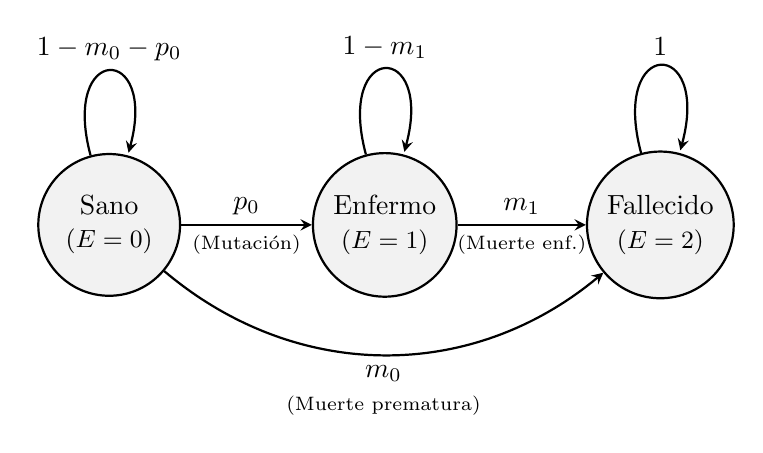
\begin{tikzpicture}[
			>=stealth, % Estilo de las flechas
			node distance=3.5cm, % Distancia entre nodos
			on grid,
			auto,
			state/.style={circle, draw=black, thick, fill=gray!10, minimum size=1.8cm, align=center}
			]
			
			% DEFINICIÓN DE LOS NODOS (ESTADOS)
			\node[state] (Sano) {Sano \\ \small($E=0$)};
			\node[state] (Enfermo) [right=of Sano] {Enfermo \\ \small($E=1$)};
			\node[state] (Fallecido) [right=of Enfermo] {Fallecido \\ \small($E=2$)};
			
			% FLECHAS DE TRANSICIÓN (RUTAS)
			\path[->, thick] 
			% Bucles sobre sí mismos (permanencia)
			(Sano) edge [loop above] node {$1 - m_0 - p_0$} (Sano)
			(Enfermo) edge [loop above] node {$1 - m_1$} (Enfermo)
			(Fallecido) edge [loop above] node {$1$} (Fallecido)
			
			% Transiciones sin retorno
			(Sano) edge node [above] {$p_0$} node [below, font=\scriptsize] {(Mutación)} (Enfermo)
			(Enfermo) edge node [above] {$m_1$} node [below, font=\scriptsize] {(Muerte enf.)} (Fallecido)
			
			% Transición directa por debajo (Muerte prematura de sano)
			(Sano) edge [bend right=40] node [below, align=center] {$m_0$ \\ \scriptsize (Muerte prematura)} (Fallecido);
			
		\end{tikzpicture}
		\caption{Grafo de transición de estados individuales en el sistema estocástico.}
		\label{fig:grafo_estados}
	\end{figure}
	
	A nivel poblacional, para todos los individuos, la dinámica se formaliza mediante un Proceso de Ramificación de Galton-Watson. 
	
	\begin{figure}[htbp]
		\centering
		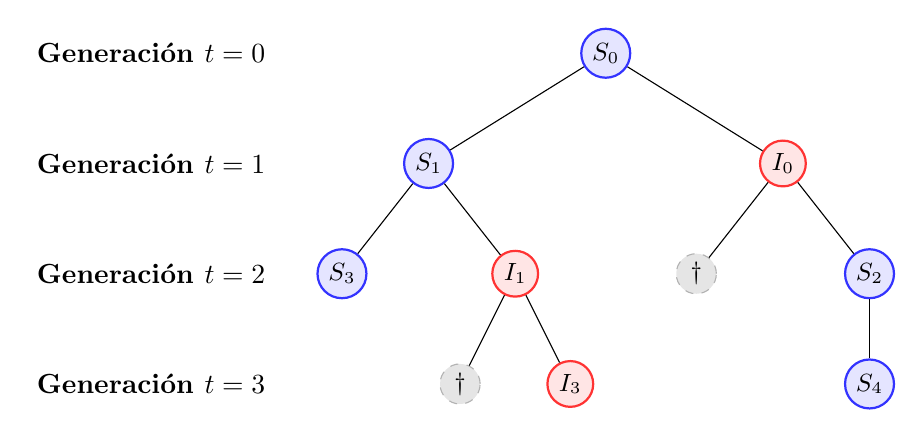
\begin{tikzpicture}[
			level 1/.style={sibling distance=4.5cm, level distance=1.4cm},
			level 2/.style={sibling distance=2.2cm, level distance=1.4cm},
			level 3/.style={sibling distance=1.4cm, level distance=1.4cm},
			sano/.style={circle, draw=blue!80, fill=blue!10, thick, inner sep=2pt, font=\small},
			enfermo/.style={circle, draw=red!80, fill=red!10, thick, inner sep=2pt, font=\small},
			muerto/.style={circle, draw=gray!60, fill=gray!20, dashed, inner sep=2pt, font=\small}
			]
			
			% Generación t=0 (Raíz)
			\node[sano] (root) {$S_0$}
			% Generación t=1
			child { node[sano] {$S_1$} 
				% Generación t=2
				child { node[sano] {$S_3$} }
				child { node[enfermo] {$I_1$} 
					% Generación t=3
					child { node[muerto] {$\dagger$} }
					child { node[enfermo] {$I_3$} }
				}
			}
			child { node[enfermo] {$I_0$}
				% Generación t=2
				child { node[muerto] {$\dagger$} }
				child { node[sano] {$S_2$} 
					% Generación t=3
					child { node[sano] {$S_4$} }
				}
			};
			
			% Leyenda de Generaciones bien separadas a la izquierda
			\node[anchor=east] at (-4.2, 0)    {\textbf{Generación $t=0$}};
			\node[anchor=east] at (-4.2, -1.4) {\textbf{Generación $t=1$}};
			\node[anchor=east] at (-4.2, -2.8) {\textbf{Generación $t=2$}};
			\node[anchor=east] at (-4.2, -4.2) {\textbf{Generación $t=3$}};
			
		\end{tikzpicture}
		\caption{Representación en árbol de ramificación de Galton-Watson multitipo a lo largo de 3 generaciones. Los nodos azules representan individuos sanos ($S$), los rojos enfermos ($I$) y los grises punteados ($\dagger$) corresponden a ramas extinguidas por muerte prematura.}
		\label{fig:arbol_galton_watson}
	\end{figure}
	
	En el ejemplo podemos ver como cada individuo puede o no estar enfermo y, dada su condición, tendrá más o menos posibilidades de fallecer, lo que determinará la posibilidad de reproducción. 
	
	\subsection{Variables y Parámetros del Modelo}
	\label{subsec:variables_parametros}
	
	Para formalizar analíticamente el comportamiento del proceso de ramificación, se definen a continuación el conjunto de variables de estado, parámetros del sistema y métricas observadas.
	
	\subsubsection{Variables de Estado Poblacionales e Individuales}
	La dinámica temporal de la población se describe a través de las siguientes variables discretas definidas en la generación $t \in \mathbb{N}_0$:
	
	\begin{itemize}
		\item $N_t \in \mathbb{N}_0$: \textbf{Tamaño total de la población viva} en la generación $t$. Representa el número de nodos activos en la generación $t$ del árbol de ramificación.
		\item $S_t \in \mathbb{N}_0$: \textbf{Población de individuos sanos} ($E=0$) en la generación $t$.
		\item $I_t \in \mathbb{N}_0$: \textbf{Población de individuos enfermos} ($E=1$) en la generación $t$. Cumple $N_t = S_t + I_t$.
		\item $E_{t,j} \in \{0, 1, 2\}$: \textbf{Estado individual} del sujeto $j$-ésimo en la generación $t$, correspondiente a Sano ($0$), Enfermo ($1$) y Fallecido ($2$).
		\item $X_{t,j} \in \mathbb{N}_0$: \textbf{Número aleatorio de descendientes} generados por el individuo $j$ que ha sobrevivido en la generación $t$.
		\item $p_{I,t} = \frac{I_t}{N_t}$: \textbf{Prevalencia de la enfermedad} en la generación $t$, que indica la proporción de individuos infectados en la población viva.
	\end{itemize}
	
	\subsubsection{Parámetros Configurables del Sistema}
	Los parámetros fijos que determinan las tasas de mortalidad, natalidad y probabilidad de transmisión condicional en el **Caso Base** se resumen en la Tabla~\ref{tab:parametros_caso_base}.
	
	\begin{table}[htbp]
		\caption{Parámetros cuantitativos definidos para el modelo estocástico en el Caso Base.}
		\label{tab:parametros_caso_base}
		\centering
		\begin{tabular}{lll}
			\hline
			\textbf{Parámetro} & \textbf{Descripción} & \textbf{Valor asignado} \\
			\hline
			$N_0$ & Tamaño inicial de la población viva & $1000$ \\
			$p_{I,0}$ & Proporción inicial de enfermos & $0.05$ ($5\%$) \\
			$\lambda$ & Parámetro de la distribución de Poisson (natalidad esperada por habitante) & $1.15$ \\
			$m_0$ & Tasa de mortalidad basal de individuos sanos & $0.05$ ($5\%$) \\
			$m_1$ & Tasa de mortalidad severa por patología (individuos enfermos) & $0.60$ ($60\%$) \\
			$p_0$ & Probabilidad de mutación \textit{de novo} (hijo enfermo de padre sano) & $0.15$ ($15\%$) \\
			$p_1$ & Probabilidad de herencia vertical (hijo enfermo de padre enfermo) & $0.95$ ($95\%$) \\
			$M$ & Número de réplicas independientes en la Simulación Monte Carlo & $500$ \\
			\hline
		\end{tabular}
	\end{table}
	
	\subsubsection{Métricas de Salida y Variables Observables}
	Dado el carácter estocástico del modelo, las métricas analíticas calculadas a partir del experimento Monte Carlo para estimar la tendencia y absorción son:
	
	\begin{itemize}
		\item $\mathbb{E}[N_t]$: \textbf{Esperanza matemática del tamaño poblacional} en la generación $t$, estimada a través del promedio de las $M=500$ trayectorias simuladas.
		\item $\text{IC}_{95\%}(N_t)$: \textbf{Intervalo de confianza al 95\%} para el tamaño poblacional medio en el tiempo $t$.
		\item $T_{\text{abs}}$: \textbf{Tiempo de absorción} (o tiempo hasta la extinción total), definido formalmente como $T_{\text{abs}} = \min \{ t \ge 0 \mid N_t = 0 \}$.
		\item $\mathbb{E}[T_{\text{abs}}]$: \textbf{Tiempo medio hasta la absorción}, calculado como el valor esperado del tiempo de extinción sobre las réplicas extinguidas.
		\item $P_{\text{ext}} = P(N_t = 0 \text{ para algún } t)$: \textbf{Probabilidad empírica de extinción}, calculada como el cociente de trayectorias que alcanzan el estado absorbente sobre el total de réplicas $M$.
		\item $\mathcal{R}_0$: \textbf{Número reproductivo efectivo}, definido como el valor esperado de descendientes supervivientes por habitante ($\mathcal{R}_{0,\text{sano}} = (1-m_0)\lambda$ y $\mathcal{R}_{0,\text{enfermo}} = (1-m_1)\lambda$).
	\end{itemize}
	
	\subsection{Probabilidad de Extinción del Caso Base}
	\label{subsec:probabilidad_extincion_caso_base}
	
	Uno de los aspectos analíticos centrales de este trabajo es la determinación de la probabilidad de extinción del Caso Base en ausencia de tratamiento.
	
	En la teoría de Procesos de Ramificación de Galton-Watson, el destino a largo plazo de la población viene determinado por el número reproductivo efectivo ($\mathcal{R}_0$), definido como el número esperado de descendientes supervivientes producidos por un individuo. Para variables aleatorias discretas de descendencia como la distribución de Poisson, la esperanza matemática se calcula como la media ponderada:
	\begin{equation}
		\mathbb{E}[X] = \sum_{k=0}^{\infty} k \cdot P(X = k) = \lambda
	\end{equation}
	
	Sin embargo, al tratarse de un proceso multitipo con dos estados vivos (sanos $E=0$ y enfermos $E=1$), el número esperado de descendientes por individuo superviviente difiere según su fenotipo:
	\begin{align}
		\mathcal{R}_{0,\text{sano}} &= (1 - m_0)\lambda = (1 - 0.05) \times 1.15 = 1.0925, \\
		\mathcal{R}_{0,\text{enfermo}} &= (1 - m_1)\lambda = (1 - 0.60) \times 1.15 = 0.46.
	\end{align}
	
	Aunque la subpoblación sana aparentemente tiene posibilidades de sobrevivir, ($\mathcal{R}_{0,\text{sano}} > 1$), la presencia de la mutación \textit{de novo} ($p_0 = 0.15$) atrae a los individuos sanos al estado enfermedad. Al ser la probabilidad de los enfermos fuertemente subcrítica ($\mathcal{R}_{0,\text{enfermo}} < 1$), el número reproductivo efectivo global del sistema decae por debajo del umbral crítico ($\mathcal{R}_0 \le 1$). 

	
	De acuerdo con el teorema fundamental de Galton-Watson, cuando el promedio de reemplazo global satisface $\mathcal{R}_0 \le 1$, la probabilidad de absorción en la extinción final es $\eta = 1.0$, garantizando que la población se extinguirá en el $100\%$ de las realizaciones a largo plazo ($P_{\text{ext}} = 1.0$).
	
	 
	\section{Caso Base: Análisis Estocástico sin Intervención}
	\label{sec:caso_base}
	En esta sección se analiza de manera experimental el caso base sin intervención, con el fin de demostrar mediante una simulación que la población acabará extinguiéndose con una probabilidad de $\eta = 1$. 
	
	\subsection{Configuración de parámetros}
	Se han seleccionado estos parámetros iniciales y se continuará con estos valores por defecto durante el resto del estudio. 
	
	\begin{itemize}
		\item \textbf{Tamaño poblacional inicial ($N_0 = 1000$):} Número total de individuos vivos en la generación $t=0$, lo que proporciona un tamaño muestral amplio para evaluar la estocasticidad demográfica.
		\item \textbf{Prevalencia inicial de la patología ($p_I = 0.05$):} Proporción inicial de enfermos respecto al total de la población en $t=0$, correspondiendo a $50$ individuos enfermos ($I_0 = 50$) y $950$ individuos sanos ($S_0 = 950$).
		\item \textbf{Tasa de natalidad esperada ($\lambda = 1.15$):} Parámetro de la distribución de Poisson ($X \sim \text{Poisson}(\lambda)$) que rige la cantidad de descendientes producidos por cada progenitor que sobrevive a la fase de reproducción.
		\item \textbf{Mortalidad basal de sanos ($m_0 = 0.05$):} Proporción de individuos sanos que fallecen prematuramente por causas ajenas a la patología antes de alcanzar la etapa reproductiva ($5\%$).
		\item \textbf{Mortalidad severa por patología ($m_1 = 0.60$):} Tasa de fallecimiento de individuos enfermos en ausencia de tratamiento farmacológico ($60\%$).
		\item \textbf{Probabilidad de mutación \textit{de novo} ($p_0 = 0.15$):} Probabilidad de que un descendiente desarrolle la enfermedad cuando su progenitor está sano ($15\%$).
		\item \textbf{Probabilidad de herencia vertical ($p_1 = 0.95$):} Probabilidad de que un descendiente herede el fenotipo patológico cuando su progenitor está enfermo ($95\%$).
		\item \textbf{Horizonte temporal ($t_{\max} = 90$):} Número máximo de generaciones discretas evaluadas por trayectoria.
	\end{itemize}
	
	
	La Tabla~\ref{tab:configuracion_parametros} resume la correspondencia entre las variables empleadas en la implementación computacional en Python y la notación formal en LaTeX utilizada en el modelo analítico.
	
	\begin{table}[htbp]
		\caption{Valores numéricos de los parámetros por defecto configurados en el modelo de Galton-Watson.}
		\label{tab:configuracion_parametros}
		\centering
		\begin{tabular}{lllc}
			\hline
			\textbf{Variable Python} & \textbf{Símbolo LaTeX} & \textbf{Descripción biológica / estadística} & \textbf{Valor asignado} \\
			\hline
			\texttt{n0} & $N_0$ & Población inicial total & $1000$ \\
			\texttt{pI} & $p_I$ & Proporción inicial de individuos enfermos & $0.05$ \\
			\texttt{lambda\_descendientes} & $\lambda$ & Parámetro de la distribución de Poisson & $1.15$ \\
			\texttt{m0} & $m_0$ & Mortalidad prematura basal (individuos sanos) & $0.05$ \\
			\texttt{m1} & $m_1$ & Mortalidad severa (individuos enfermos) & $0.60$ \\
			\texttt{p0} & $p_0$ & Probabilidad de mutación \textit{de novo} & $0.15$ \\
			\texttt{p1} & $p_1$ & Probabilidad de herencia vertical & $0.95$ \\
			\texttt{generaciones} & $t_{\max}$ & Horizonte temporal máximo de simulación & $90$ \\
			\hline
		\end{tabular}
	\end{table}
	
	\subsection{Simulación en Python}
	Con todos los parámetros seleccionados, se introducen en \textit{Python} inicializando la población con un total de 1000 individuos, mayoritariamente sanos. 
	
	Posteriormente se comienza la simulación Galton-Watson. Para cada generación se determina si fallecen o continúan reproduciendo la siguiente generación. Si continua vivo, se determina el número de descendientes y estos se clasifican (utilizando las probabilidades establecidas) como enfermos o sanos. 
	
	Se realiza esto para cada una de las generaciones. En este caso se han seleccionado 90 para que se permita visualizar la convergencia en extinción de la población. 
	
	Para la semilla \textit{1234} se obtienen los resultados presentados a continuación. 
	
	\begin{figure}[htbp]
		\centering
		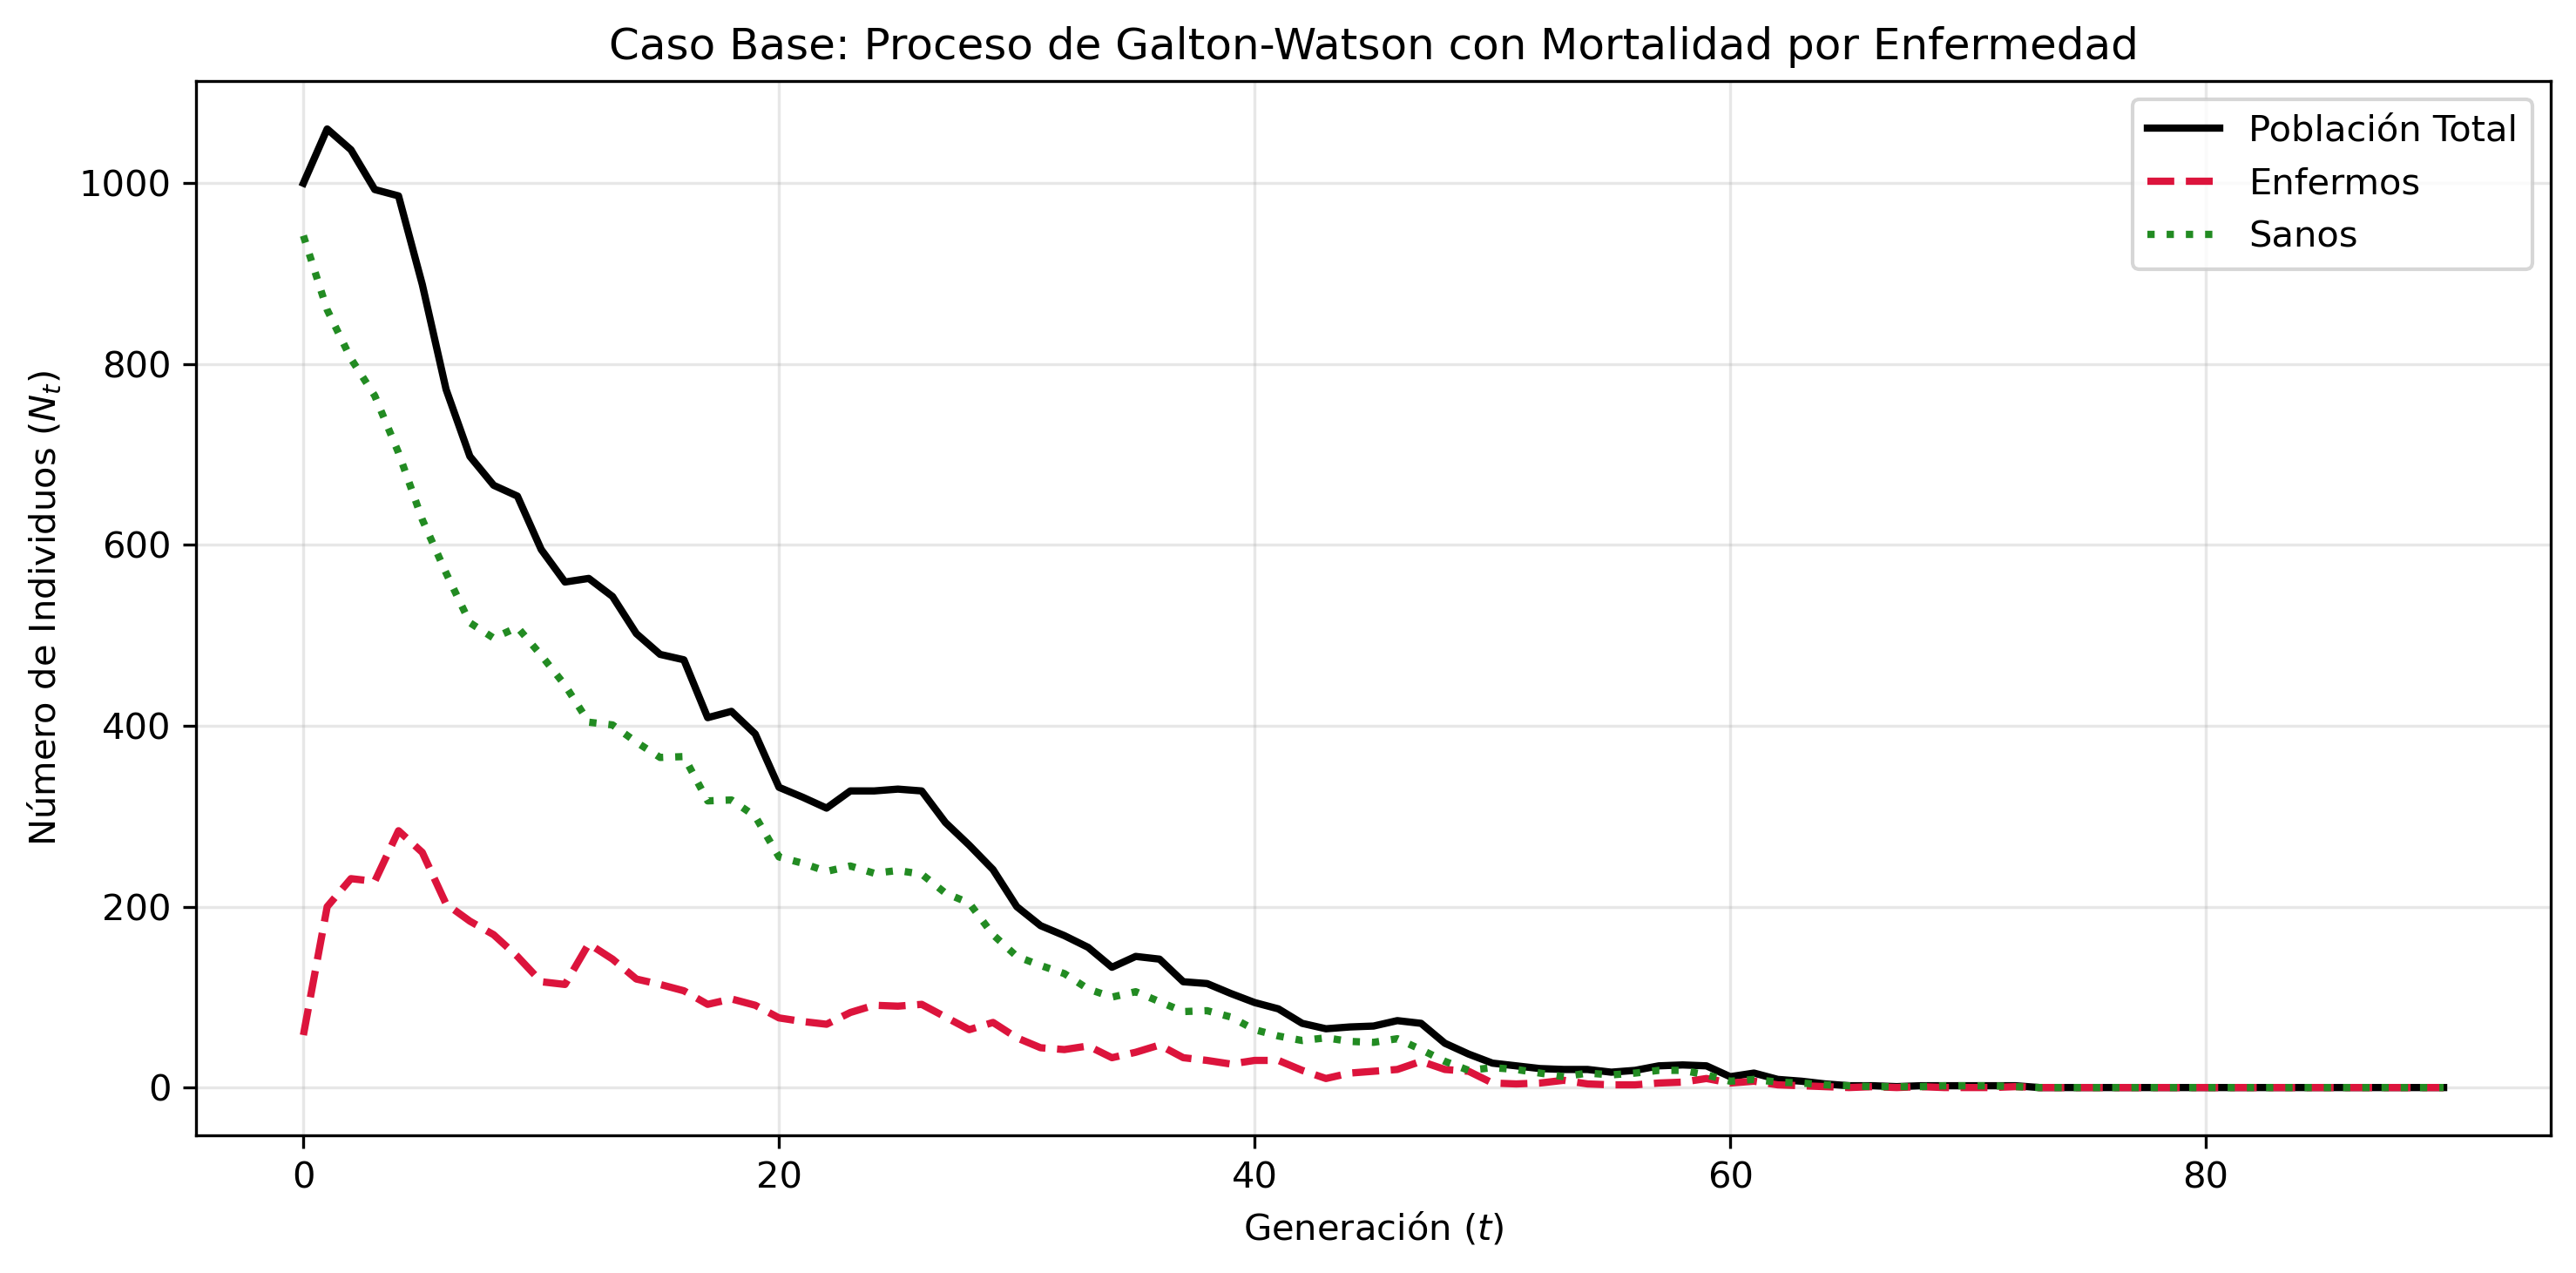
\includegraphics[width=0.85\textwidth]{../imagenes/simulacion_incial_sin_farmaco.png}
		\caption{Trayectoria temporal de la población en una única realización del Caso Base sin intervención farmacológica ($N_0=1000$, $p_I=0.05$, $\lambda=1.15$). Se observa la evolución de la población total (línea continua negra), sanos (línea punteada verde) y enfermos (línea discontinua roja) hasta la absorción en $N=0$.}
		\label{fig:simulacion_inicial_caso_base}
	\end{figure}
	
	Se observa que la población queda extinta entre 60 y 65 pasos. Primeramente el número de enfermos no es tan elevado, pero crece exponencialmente durante los primeros pasos, consiguiendo que los enfermos comiencen a morir drásticamente mientras la enfermedad sigue propagándose y el número de sanos desciende rápidamente.
	
	El motivo por el que la enfermedad se propaga tan rápido no ocurre solamente por la herencia vertical, sino también por la mutación \textit{de novo} que aumenta el número de enfermos. 
	
	\subsection{Experimento de Monte Carlo}
	En la sección anterior se estudia la trayectoria de una única simulación del Proceso de Galton-Watson. En cambio, es de nuestro interés eliminar la posible aleatoriedad que se pueda producir en cada simulación. Es por ello que se introduce la simulación de Monte Carlo, un conjunto de simulaciones que permiten observar la trayectoria media y comportamiento esperado a largo plazo. 
	
	En nuestro caso hemos seleccionado un total de 500 réplicas para la simulación. En cada iteración de las 500 réplicas se realiza una única simulación, una única trayectoria. 
	
	
	\begin{figure}[htbp]
		\centering
		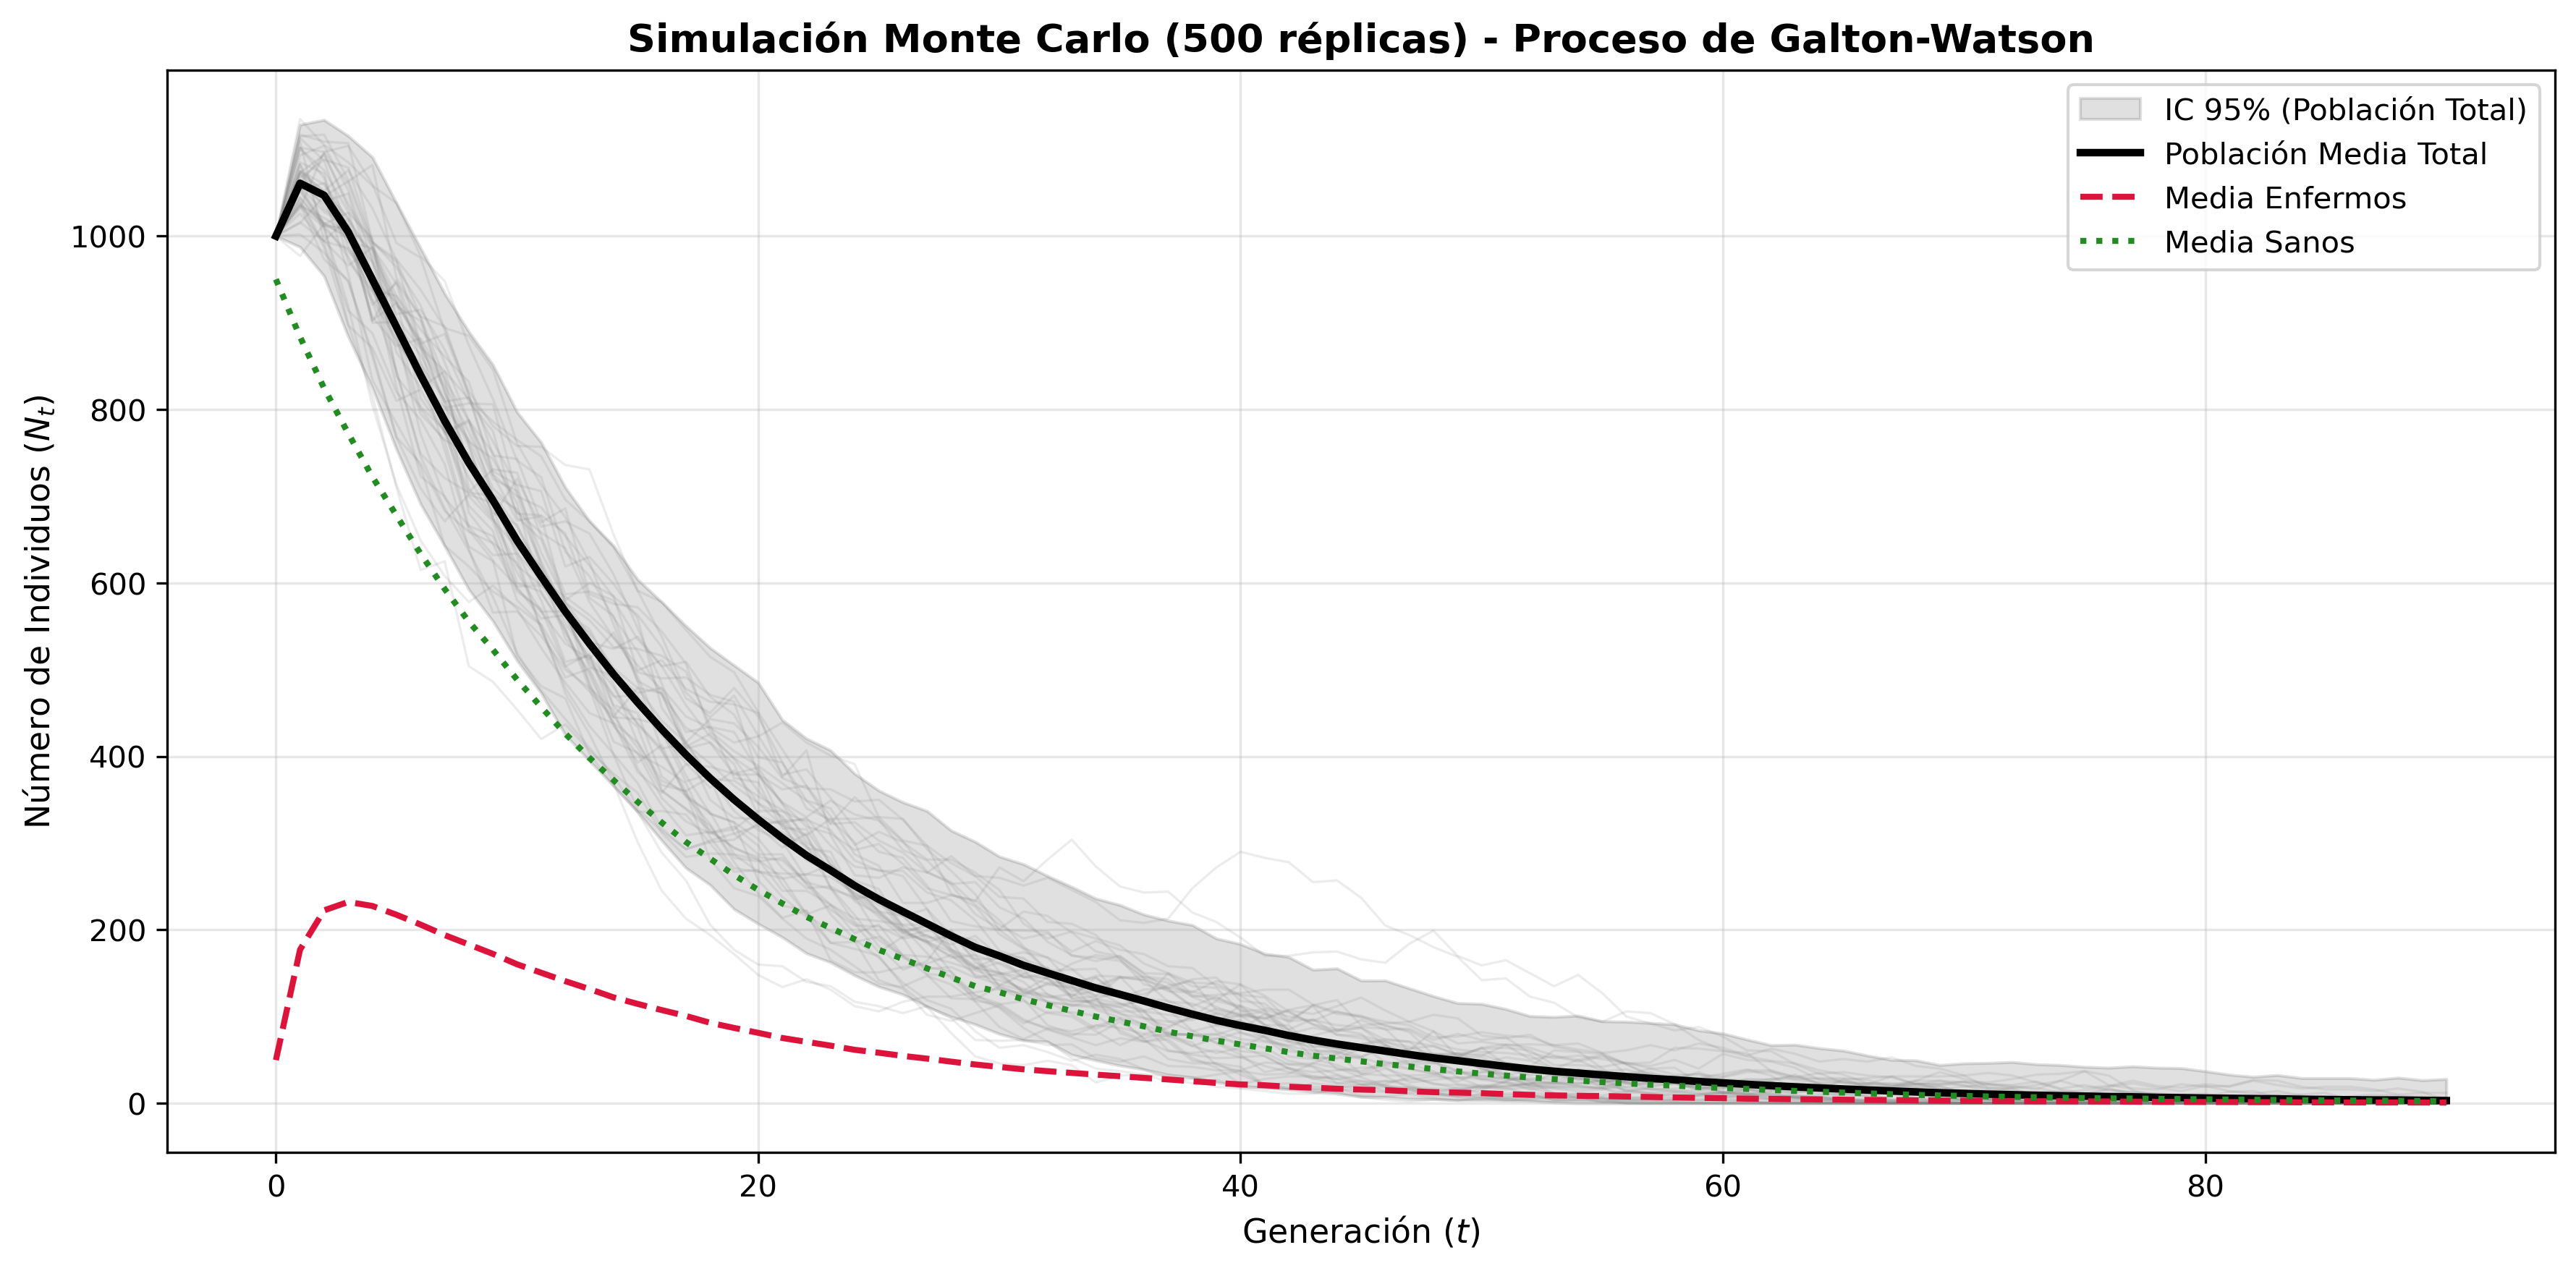
\includegraphics[width=0.85\textwidth]{../imagenes/simulacion_incial_sin_farmaco_monte_carlo.png}
		\caption{Trayectoria temporal de la población una simulación Monte Carlo de 500 réplicas de la realización del Caso Base sin intervención farmacológica ($N_0=1000$, $p_I=0.05$, $\lambda=1.15$, $B = 500$). Se observa la evolución de la población total (línea continua negra), sanos (línea punteada verde) y enfermos (línea discontinua roja) hasta la absorción en $N=0$.}
		\label{fig:simulacion_inicial_caso_base_monte_carlo}
	\end{figure}
	
	
	Para cada iteración se guardan las estadísticas del proceso, como el número de enfermos, de sanos y los tiempos de extinción. Esto nos permite obtener estadísticas más interesantes y realizar inferencias. 
	
	En la Tabla 3 se pueden observar los resultados resultados estadísticos de la simulación. 
	
	\begin{table}[htbp]
		\caption{Estadísticos descriptivos del régimen de absorción y distribución del tiempo de extinción ($T_{\text{abs}}$) obtenidos en $M = 500$ réplicas de Monte Carlo ($t_{\max} = 90$).}
		\label{tab:resultados_monte_carlo}
		\centering
		\begin{tabular}{lc}
			\hline
			\textbf{Métrica / Estadístico} & \textbf{Valor Observado} \\
			\hline
			Número total de réplicas ($M$) & $500$ \\
			Trayectorias extinguidas ($N_t = 0$) & $355$ \\
			Ratio empírico de extinción ($P_{\text{ext}}$ a $t=90$) & $71.00\%$ \\
			\hline
			Tiempo medio de absorción ($\mathbb{E}[T_{\text{abs}}]$) & $71.94$ generaciones \\
			Mediana del tiempo de absorción & $72.00$ generaciones \\
			Desviación típica ($\sigma$) & $\pm 9.67$ generaciones \\
			Mínimo tiempo de absorción registrado & $46.00$ generaciones \\
			Máximo tiempo de absorción registrado & $89.00$ generaciones \\
			Primer cuartil ($\text{Q}_1$, Percentil 25) & $65.00$ generaciones \\
			Tercer cuartil ($\text{Q}_3$, Percentil 75) & $79.50$ generaciones \\
			\hline
		\end{tabular}
	\end{table}
	
	A primera vista puede verse que no todas las generaciones se han extinguido, mientras que anteriormente hemos visto que según del Proceso de Ramificación de Galton-Watson la probabilidad de absorción era de $\eta = 1$. No significa que haya habido un error, sino que la probabilidad de absorción teórica se calcula en un marco infinito, mientras que en nuestra simulación práctica solamente tenemos 90 generaciones. Esto quiere decir que precisamente nuestro resultado demuestra lo estudiado anteriormente, si realizásemos este experimento infinitas veces, la probabilidad de extinción de la población converge al $100\%$. 
	
	Otro de los resultados más interesantes es el tiempo medio de absorción. No solamente interesa estudiar si se extingue o no, sino cuantos pasos, en este caso generaciones, transcurren hasta la extinción. En este caso es de tan solo 72 generaciones, que teniendo en cuenta que la media de reproducción es de aproximadamente 25 años, esto significaría que la población que extingue en 1800 años. Teniendo en cuenta el tiempo que lleva el ser humano en la tierra en comparación con los 1800 años, significaría que puede acabar con la población en bastante poco tiempo. 
	
	\section{Evaluación del Impacto Farmacológico (Experimentos Comparativos)}
	\label{sec:farmacos}
	En esta sección se introducen varias estrategias farmacológicas. El objetivo de estas nuevas estrategias es tratar de detener la expansión de la enfermedad, evitando que se siga propagando hasta acabar en estado de absorción irremediable. 
	
	Se van a proponer un total de tres medicamentos diferentes, cada uno de ellos con una probabilidad curativa diferente para así poder estudiar diferentes casos y analizar las diferencias entre cada uno. 
	
	\subsection{Diseño de escenarios terapéuticos y modificación del modelo}
	Al introducir un fármaco, se introducen dos parámetros nuevos en el modelo: 
	\begin{itemize}
		\item $\alpha$: La eficacia terapéutica del fármaco. Cuantifica la capacidad del tratamiento para mitigar la letalidad asociada a la patología en individuos afectados. Define una nueva mortalidad efectiva bajo el tratamiento. 
		\begin{equation}
			m_{1,\text{trat}} = m_1 \cdot (1 - \alpha)
		\end{equation}
		De este modo, cuando $\alpha = 0$ el fármaco es inactivo (recuperando el escenario del Caso Base $m_{1,\text{trat}} = m_1$), mientras que un valor de $\alpha = 1$ implica una protección completa frente a la mortalidad específica de la enfermedad ($m_{1,\text{trat}} = 0$).
		\item $\rho$: La tasa de curación de los individuos. Probabilidad condicional de que un individuo enfermo que logra sobrevivir a la etapa de selección ($1 - m_{1,\text{trat}}$) experimente una remisión completa de la patología, transitando de vuelta al estado sano ($E=0$) antes de iniciar la fase reproductiva. Esta variable rompe la irreversibilidad del grafo original al habilitar una transición de retorno ($E=1 \rightarrow E=0$), lo que implica que dicho individuo pasará a reproducirse bajo las tasas de transmisión de un progenitor sano ($p_0$) en lugar de la herencia vertical ($p_1$).
	\end{itemize}
		
	Con estos nuevos parámetros introducidos, el diagrama de estados del modelo cambia por completo tal y como se muestra en la siguiente figura.  
	
	\begin{figure}[htbp]
		\centering
		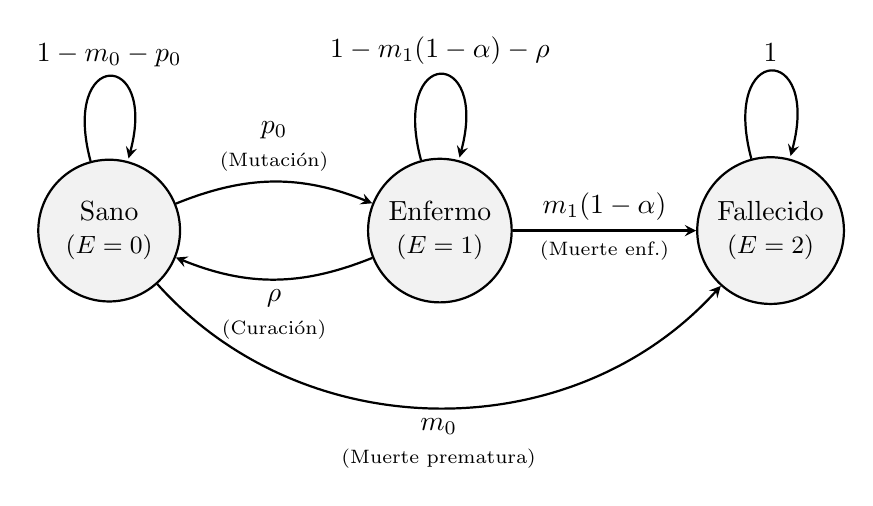
\begin{tikzpicture}[
			>=stealth, % Estilo de las flechas
			node distance=4.2cm, % Mayor separación para evitar solapamientos
			on grid,
			auto,
			state/.style={circle, draw=black, thick, fill=gray!10, minimum size=1.8cm, align=center}
			]
			
			% DEFINICIÓN DE LOS NODOS (ESTADOS)
			\node[state] (Sano) {Sano \\ \small($E=0$)};
			\node[state] (Enfermo) [right=of Sano] {Enfermo \\ \small($E=1$)};
			\node[state] (Fallecido) [right=of Enfermo] {Fallecido \\ \small($E=2$)};
			
			% FLECHAS DE TRANSICIÓN (RUTAS)
			\path[->, thick] 
			% Bucles sobre sí mismos (permanencia)
			(Sano) edge [loop above] node {$1 - m_0 - p_0$} (Sano)
			(Enfermo) edge [loop above] node[align=center] {$1 - m_1(1-\alpha) - \rho$} (Enfermo)
			(Fallecido) edge [loop above] node {$1$} (Fallecido)
			
			% Transición Sano -> Enfermo (curvada por arriba para no chocar con el retorno)
			(Sano) edge [bend left=22] node [above, align=center] {$p_0$ \\ \scriptsize (Mutación)} (Enfermo)
			
			% Nueva transición de retorno: Enfermo -> Sano (Curación)
			(Enfermo) edge [bend left=22] node [below, align=center] {$\rho$ \\ \scriptsize (Curación)} (Sano)
			
			% Transición Enfermo -> Fallecido modificada por eficacia alpha
			(Enfermo) edge node [above] {$m_1(1-\alpha)$} node [below, font=\scriptsize] {(Muerte enf.)} (Fallecido)
			
			% Transición directa por debajo (Muerte prematura de sano)
			(Sano) edge [bend right=48] node [below, align=center] {$m_0$ \\ \scriptsize (Muerte prematura)} (Fallecido);
			
		\end{tikzpicture}
		\caption{Grafo de transición de estados individuales bajo intervención farmacológica. Se incorpora la tasa de curación ($\rho$) como transición reversible hacia el estado sano y la reducción de la mortalidad patológica mediante la eficacia terapéutica ($m_1(1-\alpha)$).}
		\label{fig:grafo_estados_farmaco}
	\end{figure}

	
	La principal diferencia, como se comentaba anteriormente, es que ahora el enlace del estado \textit{Sano} a \textit{Enfermo} es bidireccional, por lo que existe una probabilidad de $\rho$ de volver al estado inicial de \textit{Sano}, permitiendo así que se continúe con la fase reproductiva del individuo y tratando de impedir la extinción de la población. 
	
	
	\subsection{Definición de los Escenarios Terapéuticos}
	Con el objetivo de analizar la sensibilidad del sistema ante distintos niveles de potencia clínica, se definen tres escenarios farmacológicos independientes manteniendo constantes los parámetros demográficos del Caso Base ($N_0 = 1000$, $p_I = 0.05$, $\lambda = 1.15$, $m_0 = 0.05$, $m_1 = 0.60$, $p_0 = 0.15$ y $p_1 = 0.95$). Los valores asignados a cada tratamiento se detallan en la Tabla~\ref{tab:escenarios_farmacos}.
	
	\begin{table}[htbp]
		\caption{Configuración de los parámetros terapéuticos ($\alpha$ y $\rho$) y mortalidad efectiva resultante para los tres fármacos evaluados.}
		\label{tab:escenarios_farmacos}
		\centering
		\begin{tabular}{llccc}
			\hline
			\textbf{Escenario} & \textbf{Perfil Terapéutico} & \textbf{Eficacia ($\alpha$)} & \textbf{Curación ($\rho$)} & \textbf{Mortalidad ($m_{1,\text{trat}}$)} \\
			\hline
			Caso Base & Sin intervención médica & $0.00$ & $0.00$ & $0.600$ \\
			Fármaco 1 & Tratamiento paliativo / eficacia baja & $0.30$ & $0.10$ & $0.420$ \\
			Fármaco 2 & Tratamiento estándar / eficacia media & $0.60$ & $0.35$ & $0.240$ \\
			Fármaco 3 & Terapia curativa / eficacia alta & $0.85$ & $0.70$ & $0.090$ \\
			\hline
		\end{tabular}
	\end{table}
	
	La relación entre la eficacia y la mortalidad es inversa, a mayor eficacia del fármaco, menor será la nueva tasa de mortalidad bajo el tratamiento en los individuos. A su vez, cuando mayor sea la tasa de curación, menor será el ratio de enfermos registrados, por lo que su propagación decrecerá. 
	
	\begin{equation}
		m_{1,\text{trat}}(\alpha) = m_1 \cdot (1 - \alpha)
	\end{equation}
	\begin{equation}
		I_{t,\text{trat}}(\rho) = I_t \cdot (1 - m_{1,\text{trat}}) \cdot (1 - \rho)
	\end{equation}
	
	En el contexto práctico y ficticio en el que se desarrolla este proyecto, se puede permitir experimentar con diferentes valores. En cambio, en la vida real bajo un contexto de una enfermedad real que se está propagando, no es tan fácil encontrar fármacos que sean perfectos. Es complicado desarrollar tratamientos con una eficacia y una curación muy elevada, por eso mismo se tratará de simular un entorno clínico realista proponiendo tres medicamentos con diferentes tasas de eficacia y curación para mostrar las diferencias evolutivas en la población. 
	
	\subsection{Estudio de las nuevas probabilidades de absorción de los tres modelos}
	\label{subsec:estudio_absorcion_modelos}
	
	Generalizando la función generatriz de probabilidades del proceso de Galton-Watson estándar ($\eta = \sum_{k} P(Y=k)\eta^k$) al espacio de tipos activos $E_{\text{act}} = \{\text{Sano}, \text{Enfermo}\}$, se obtiene un sistema acoplado de dos ecuaciones donde $\eta_S$ y $\eta_I$ representan las probabilidades de extinción de un linaje iniciado por un individuo sano o enfermo, respectivamente:
	
	\begin{align}
		\eta_S &= \sum_{k_S=0}^{\infty} \sum_{k_I=0}^{\infty} P_S(k_S, k_I) \, \eta_S^{k_S} \eta_I^{k_I} = \exp\Big( M_{00}(\eta_S - 1) + M_{01}(\eta_I - 1) \Big), \\
		\eta_I &= \sum_{k_S=0}^{\infty} \sum_{k_I=0}^{\infty} P_I(k_S, k_I) \, \eta_S^{k_S} \eta_I^{k_I} = \exp\Big( M_{10}(\eta_S - 1) + M_{11}(\eta_I - 1) \Big).
	\end{align}
	
	Dado que en la generación inicial $t=0$ cada uno de los $N_0 = 1000$ individuos adquiere el estado enfermo de forma independiente con probabilidad $p_I = 0.05$ (permaneciendo sano con probabilidad $1 - p_I = 0.95$), la probabilidad de extinción de un individuo inicial arbitrario es $(1 - p_I)\eta_S + p_I\eta_I$. Por independencia entre linajes, la probabilidad teórica de extinción total de la población ($\eta_{\text{total}}$) se calcula mediante:
	\begin{equation}
		\eta_{\text{total}} = \Big( (1 - p_I)\eta_S + p_I\eta_I \Big)^{N_0} = \big( 0.95\,\eta_S + 0.05\,\eta_I \big)^{1000}
	\end{equation}
	
	Sustituyendo los parámetros base ($\lambda = 1.15$, $m_0 = 0.05$, $p_0 = 0.15$) junto con las tasas modificadas $m_{1,\text{trat}} = m_1(1-\alpha)$ y $p_{1,\text{trat}} = (1-\rho)p_1 + \rho p_0$, se resuelven analíticamente los tres escenarios terapéuticos.
	
	\begin{center}
		\fcolorbox{black!60}{gray!8}{%
			\parbox{0.94\textwidth}{%
				\small
				\textbf{Nota teórica (Cálculo del número reproductivo efectivo global $\mathcal{R}_0^{\text{global}}$):} 
				En un proceso multitipo, la tasa de crecimiento asintótico de la población viene dada por el autovalor dominante de la matriz $\mathbf{M}$. Para el caso bidimensional $E_{\text{act}} = \{\text{Sano}, \text{Enfermo}\}$, este umbral crítico se obtiene analíticamente a partir de la traza ($\text{Tr}(\mathbf{M}) = M_{00} + M_{11}$) y el determinante ($\det(\mathbf{M}) = M_{00}M_{11} - M_{01}M_{10}$) mediante la expresión:
				\begin{equation*}
					\mathcal{R}_0^{\text{global}} = \frac{\text{Tr}(\mathbf{M}) + \sqrt{\big(\text{Tr}(\mathbf{M})\big)^2 - 4\det(\mathbf{M})}}{2}
				\end{equation*}
				\begin{itemize}
					\item $\mathcal{R}_0^{\text{global}} \le 1$: La población decae hacia la extinción segura ($\eta_{\text{total}} = 1$). 
					\item $\mathcal{R}_0^{\text{global}} > 1$: El sistema entra en régimen supercrítico y crece asintóticamente. Esto significa que no podemos asegurar que la población se vaya a extinguir, $\eta < 1$. 
				\end{itemize}
			}%
		}
	\end{center}
	
	\subsubsection{Modelo 1: Fármaco de Eficacia Baja ($\alpha = 0.30, \, \rho = 0.10$)}
	En este escenario, la mortalidad patológica se reduce a $m_{1,\text{trat}} = 0.420$ y la probabilidad de transmisión efectiva desciende a $p_{1,\text{trat}} = 0.870$. La matriz de medias generacionales resultante es:
	\begin{equation}
		\mathbf{M}_1 = \begin{pmatrix}
			0.9286 & 0.1639 \\
			0.0867 & 0.5803
		\end{pmatrix}
	\end{equation}
	Evaluando su autovalor dominante se obtiene un número reproductivo efectivo global de $\mathcal{R}_0^{\text{global}} = 0.9655 < 1$ (régimen subcrítico). El sistema de ecuaciones generatrices queda definido por:
	\begin{align}
		\eta_S &= \exp\Big( 0.9286(\eta_S - 1) + 0.1639(\eta_I - 1) \Big), \\
		\eta_I &= \exp\Big( 0.0867(\eta_S - 1) + 0.5803(\eta_I - 1) \Big).
	\end{align}
	La única solución en $[0,1]^2$ es $\eta_S = 1.0000$ y $\eta_I = 1.0000$, lo que conduce a una probabilidad de extinción global de:
	\begin{equation}
		\eta_{\text{total}} = \big( 0.95(1.0000) + 0.05(1.0000) \big)^{1000} = 1.0000 \quad (100\%)
	\end{equation}
	Por tanto, el Fármaco 1 retrasa el colapso poblacional pero no evita la extinción asintótica.
	
	\subsubsection{Modelo 2: Fármaco de Eficacia Intermedia ($\alpha = 0.60, \, \rho = 0.35$)}
	Al incrementar la potencia terapéutica, la mortalidad efectiva cae a $m_{1,\text{trat}} = 0.240$ y la transmisión vertical efectiva se reduce hasta $p_{1,\text{trat}} = 0.670$, generando la matriz de medias:
	\begin{equation}
		\mathbf{M}_2 = \begin{pmatrix}
			0.9286 & 0.1639 \\
			0.2884 & 0.5856
		\end{pmatrix}
	\end{equation}
	Su autovalor dominante cruza el umbral crítico situándose en $\mathcal{R}_0^{\text{global}} = 1.0340 > 1$ (régimen supercrítico). El sistema acoplado correspondiente es:
	\begin{align}
		\eta_S &= \exp\Big( 0.9286(\eta_S - 1) + 0.1639(\eta_I - 1) \Big), \\
		\eta_I &= \exp\Big( 0.2884(\eta_S - 1) + 0.5856(\eta_I - 1) \Big).
	\end{align}
	Resolviendo numéricamente el punto fijo se obtienen probabilidades individuales estrictamente inferiores a la unidad: $\eta_S = 0.9304$ y $\eta_I = 0.9542$. Al evaluar la población inicial completa de $N_0 = 1000$ sujetos, la probabilidad de absorción global resulta virtualmente nula:
	\begin{equation}
		\eta_{\text{total}} = \big( 0.95(0.9304) + 0.05(0.9542) \big)^{1000} \approx 1.63 \times 10^{-31} \approx 0
	\end{equation}
	En consecuencia, el Fármaco 2 logra revertir el colapso y garantiza la supervivencia indefinida de la población.
	
	\subsubsection{Modelo 3: Fármaco de Eficacia Alta ($\alpha = 0.85, \, \rho = 0.70$)}
	En el escenario de alta potencia curativa, la mortalidad asociada a la enfermedad se reduce a $m_{1,\text{trat}} = 0.090$ y la transmisión efectiva desciende a $p_{1,\text{trat}} = 0.390$. La matriz de medias generacionales asociada es:
	\begin{equation}
		\mathbf{M}_3 = \begin{pmatrix}
			0.9286 & 0.1639 \\
			0.6384 & 0.4081
		\end{pmatrix}
	\end{equation}
	El autovalor dominante asciende hasta $\mathcal{R}_0^{\text{global}} = 1.0835 > 1$, consolidando un régimen fuertemente supercrítico. El sistema de ecuaciones generatrices viene dado por:
	\begin{align}
		\eta_S &= \exp\Big( 0.9286(\eta_S - 1) + 0.1639(\eta_I - 1) \Big), \\
		\eta_I &= \exp\Big( 0.6384(\eta_S - 1) + 0.4081(\eta_I - 1) \Big).
	\end{align}
	La solución no trivial de punto fijo arroja $\eta_S = 0.8485$ y $\eta_I = 0.8560$. Para el conjunto de la población inicial, la probabilidad teórica de extinción es:
	\begin{equation}
		\eta_{\text{total}} = \big( 0.95(0.8485) + 0.05(0.8560) \big)^{1000} \approx 7.03 \times 10^{-72} \approx 0
	\end{equation}
	Este tercer modelo asegura una expansión demográfica sostenida y el control efectivo de la patología.
	
	\section{Simulación de las tres estrategias farmacológicas}
	La realización de las tres simulaciones de las diferentes estrategias farmacológicas mantiene la estructura algorítmica respecto a la del caso base. Las modificaciones del código \textit{Python} han sido las siguientes: 
	\begin{itemize}
		\item Modificar la probabilidad de muerte del enfermo de $m_1$ a $m_1*(1-\alpha)$. 
		\item Añadir la probabilidad $\rho$ de tal forma que si se obtiene $p < \rho$ entonces el enfermo transiciona a estado sano. 
		\item Cambiar los valores de $\alpha$ y $\rho$ para cada uno de los tres fármacos utilizados en cada experimento. 
	\end{itemize}
	
	A continuación se presentan los diferentes resultados obtenidos. 
	
	\subsection{Resultados de la utilización del primer fármaco}
	En la representación de una única trayectoria utilizando el primero de los fármacos se ve que continúa entrando en un estado de absorción permanente. 
	\begin{figure}[htbp]
		\centering
		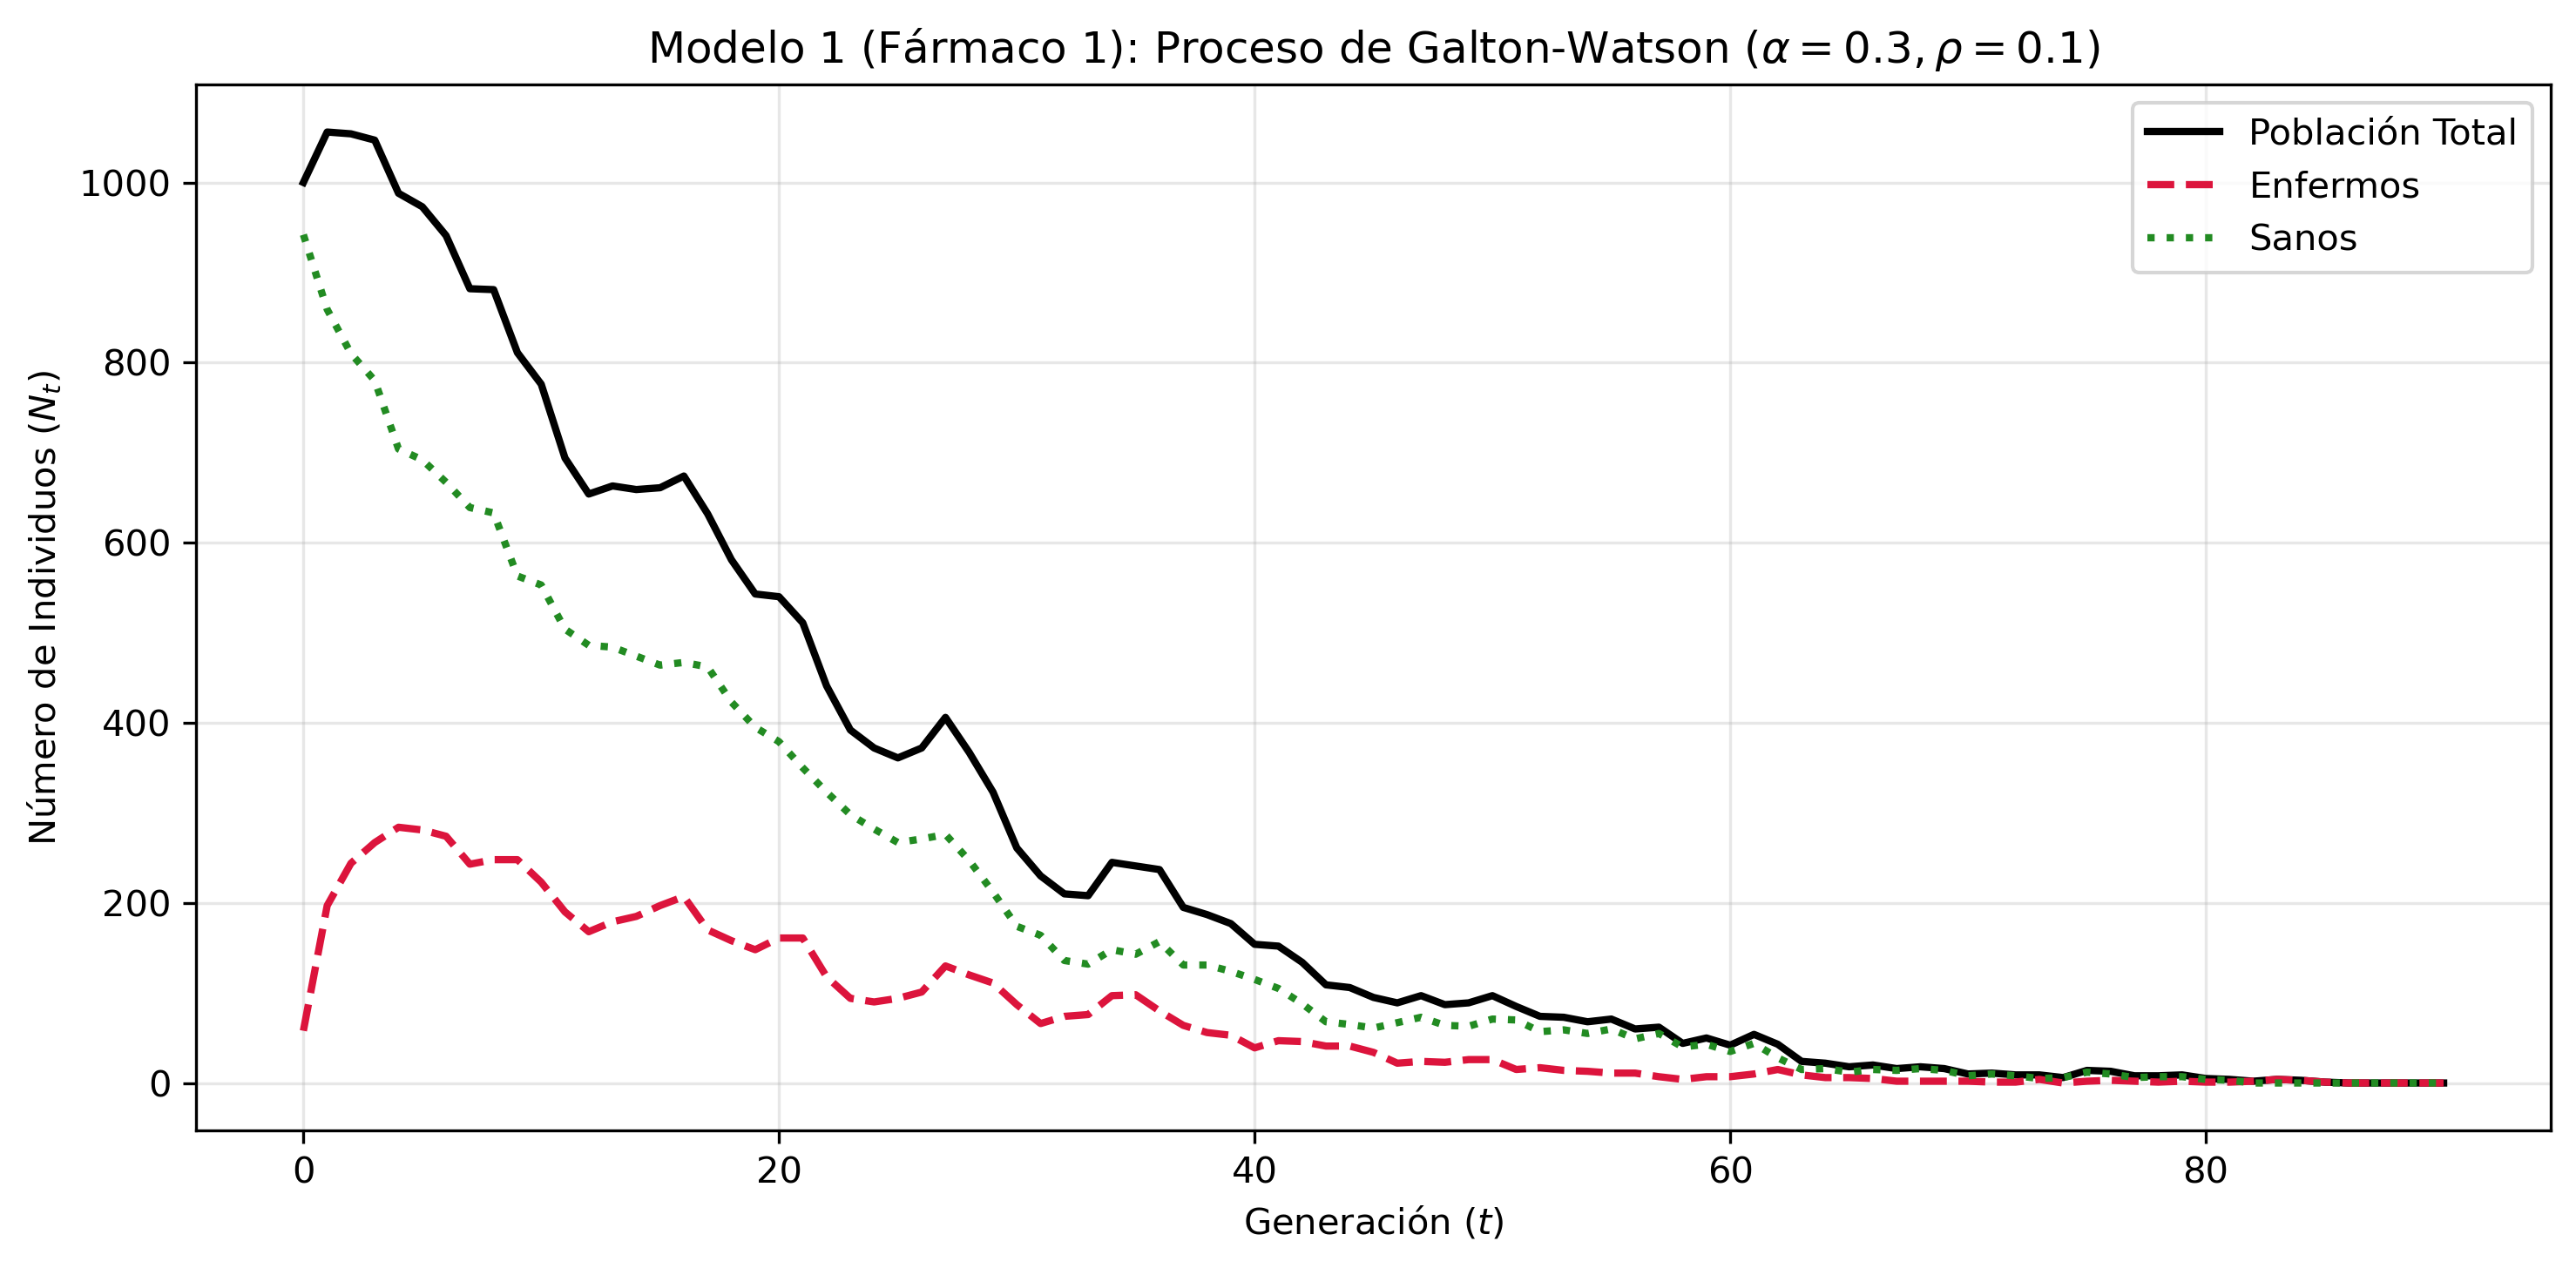
\includegraphics[width=0.85\textwidth]{../imagenes/simulacion_farmaco_1.png}
		\caption{Trayectoria temporal de la población en una única realización con el primer fármaco ($N_0=1000$, $p_I=0.05$, $\lambda=1.15$, $\alpha=0.3$, $\rho=0.1$). Se observa la evolución de la población total (línea continua negra), sanos (línea punteada verde) y enfermos (línea discontinua roja) hasta la absorción en $N=0$.}
		\label{fig:simulacion_caso_farmaco_1}
	\end{figure}
	
	En cambio, en la representación del Caso Base sin uso de fármacos se observa que, aunque también se alcanza el estado de absorción, se hace antes que con el uso de fármacos. 
	\begin{itemize}
		\item Caso Base: Se extingue aproximadamente en 60 generaciones. 
		\item Caso primer fármaco: Se extinge aproximadamente en 80 generaciones. 
	\end{itemize}
	
	Para poder sacar conclusiones más exactas eliminando al máximo la variabilidad estocástica, se realiza una simulación Monte Carlo con $M = 500$ réplicas. A continuación se muestra la figura con los resultados obtenidos. 
	
	
	\begin{figure}[htbp]
		\centering
		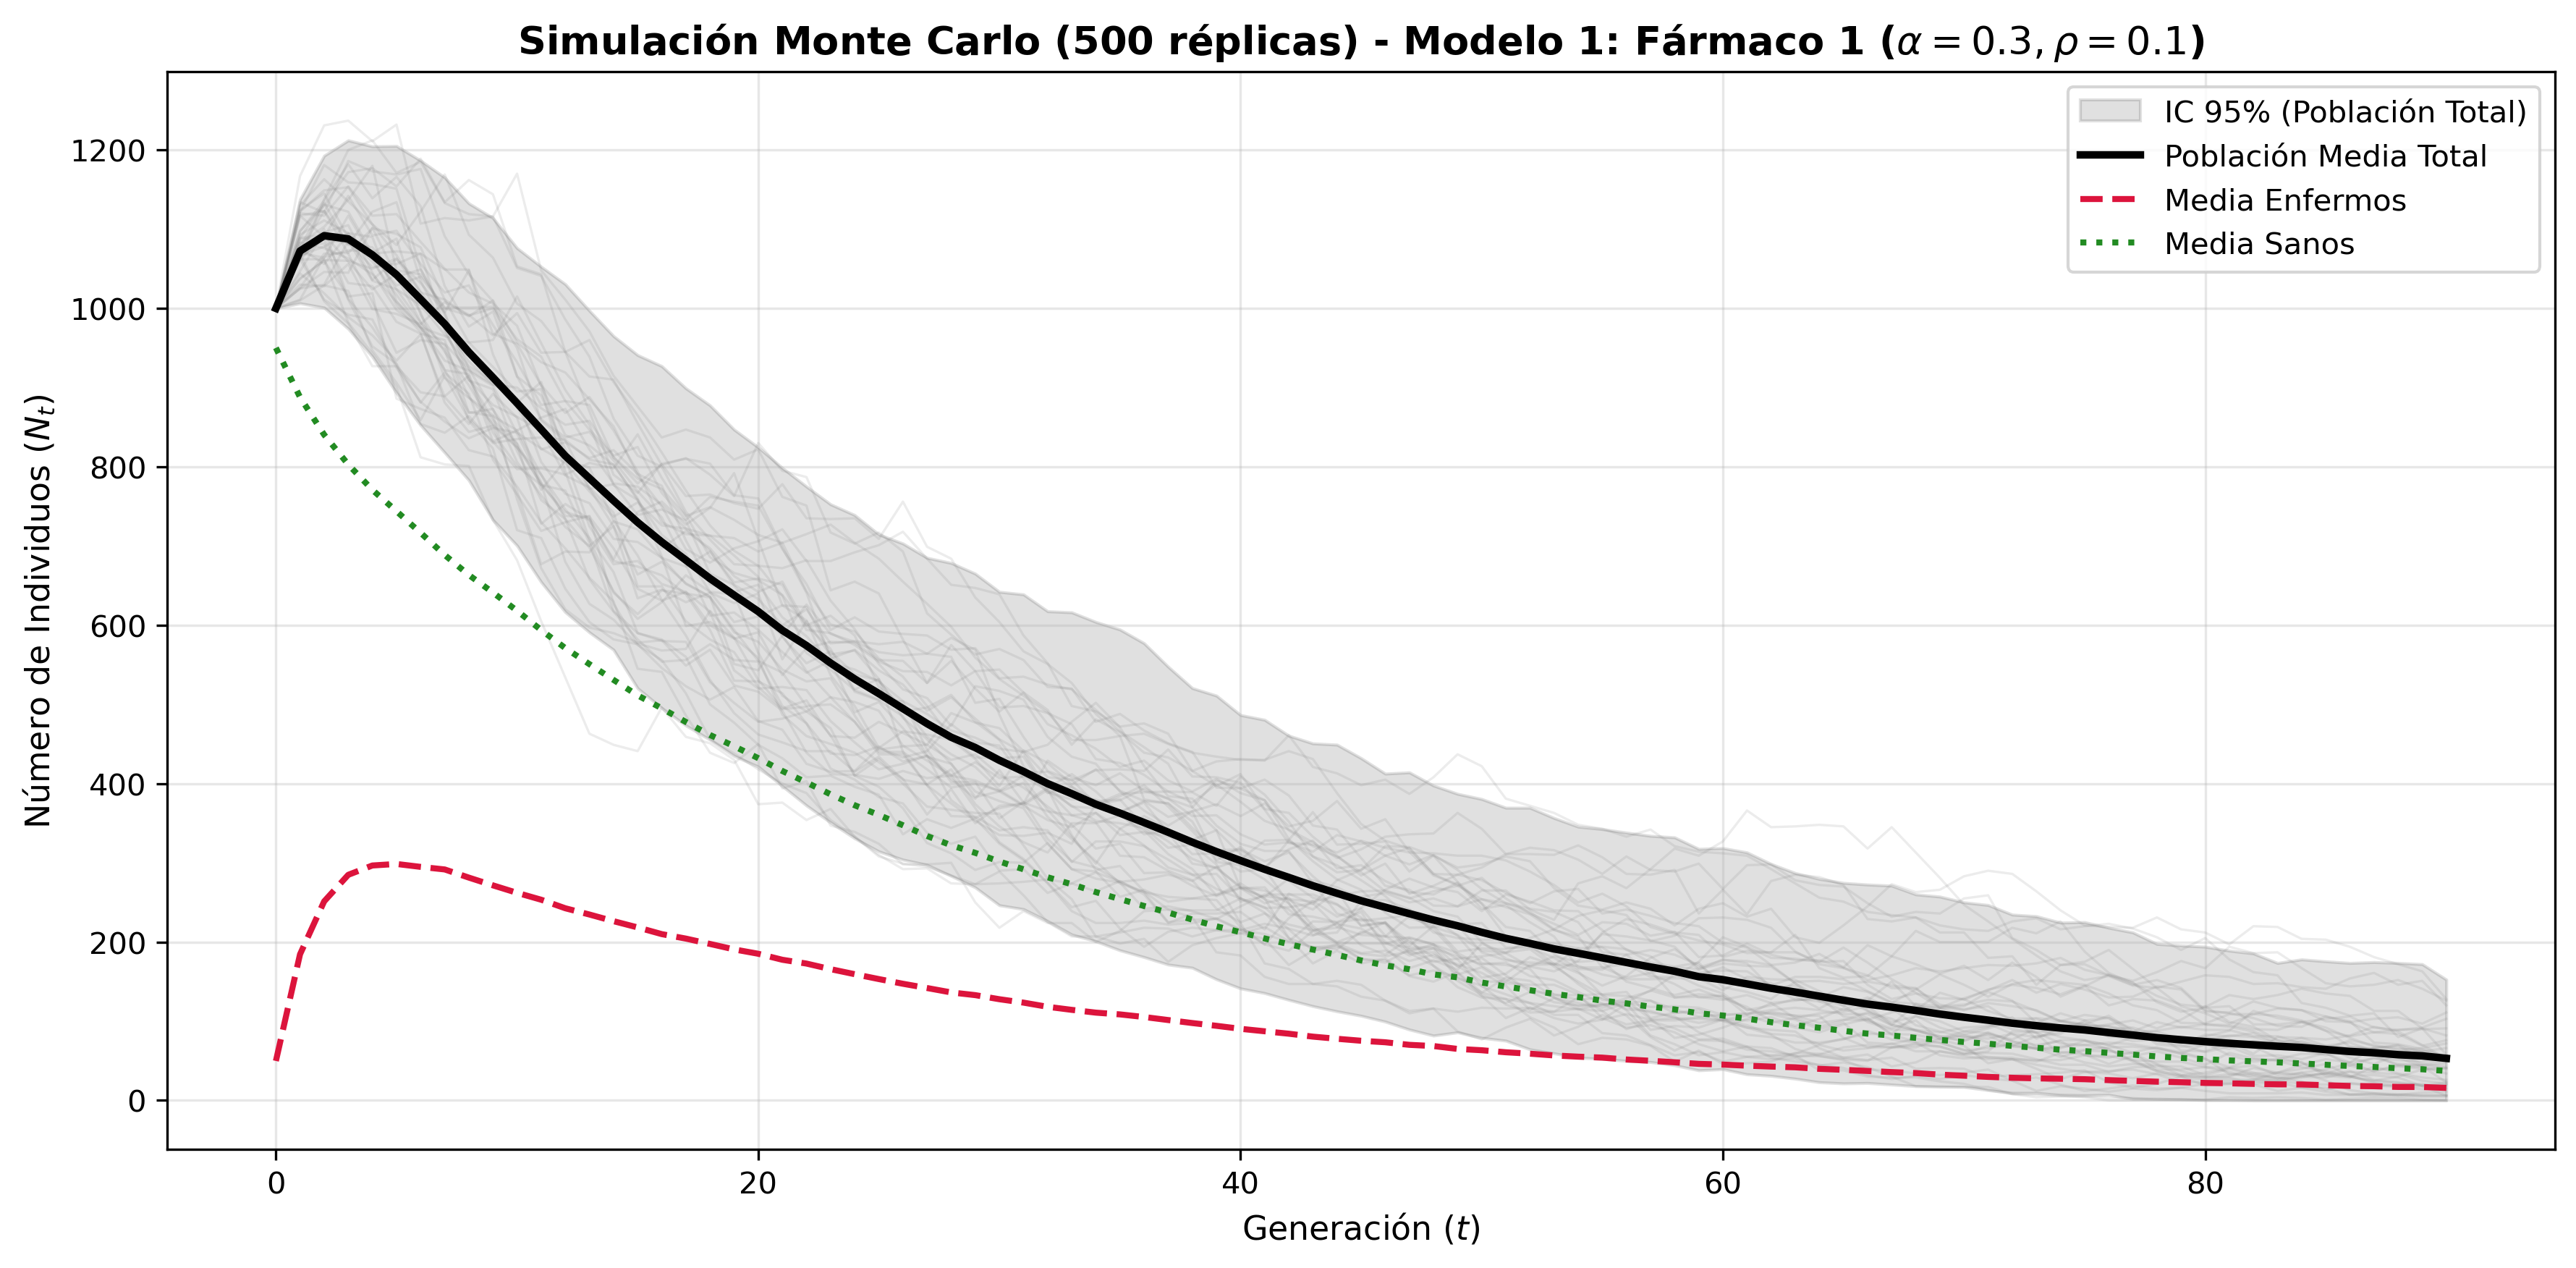
\includegraphics[width=0.85\textwidth]{../imagenes/simulacion_farmaco_1_monte_carlo.png}
		\caption{Trayectoria temporal de la población en múltiples realizaciones con el método de Monte Carlo con el primer fármaco ($N_0=1000$, $p_I=0.05$, $\lambda=1.15$, $\alpha=0.3$, $\rho=0.1$). Se observa la evolución de la población total (línea continua negra), sanos (línea punteada verde) y enfermos (línea discontinua roja) hasta la absorción en $N=0$.}
		\label{fig:simulacion_caso_farmaco_1_monte_carlo}
	\end{figure}
	
	Aunque no se llega a ver justamente la generación en la que se extingue la población porque el horizonte llega hasta $\text{t}_{max} = 90$ se puede intuir que es cerca de 110 generaciones. En el Caso Base era cercano a la generación número 75, por lo que la esperanza del tiempo de absorción ha aumentado casi un $50\%$. 
	\begin{equation}
		\text{Incremento}_1 = 100*(110 / 75 - 1) = 46.67\%
	\end{equation}
	
	En definitiva, el uso de este fármaco no será capaz de evitar la extinción de la población, pero sí retrasarlo. Teniendo en cuenta que la edad media para tener hijos es de 25 años, podría suponer un retraso de aproximadamente 850-900 años en cuanto a la extinción de la población. 
	
	\subsection{Resultados de la utilización del segundo fármaco}
	En el segundo de los casos, al utilizar otro fármaco diferente con una eficacia y una curación mucho más elevadas, se observa que, ahora sí, no se extingue la población. 
	
	\begin{figure}[htbp]
		\centering
		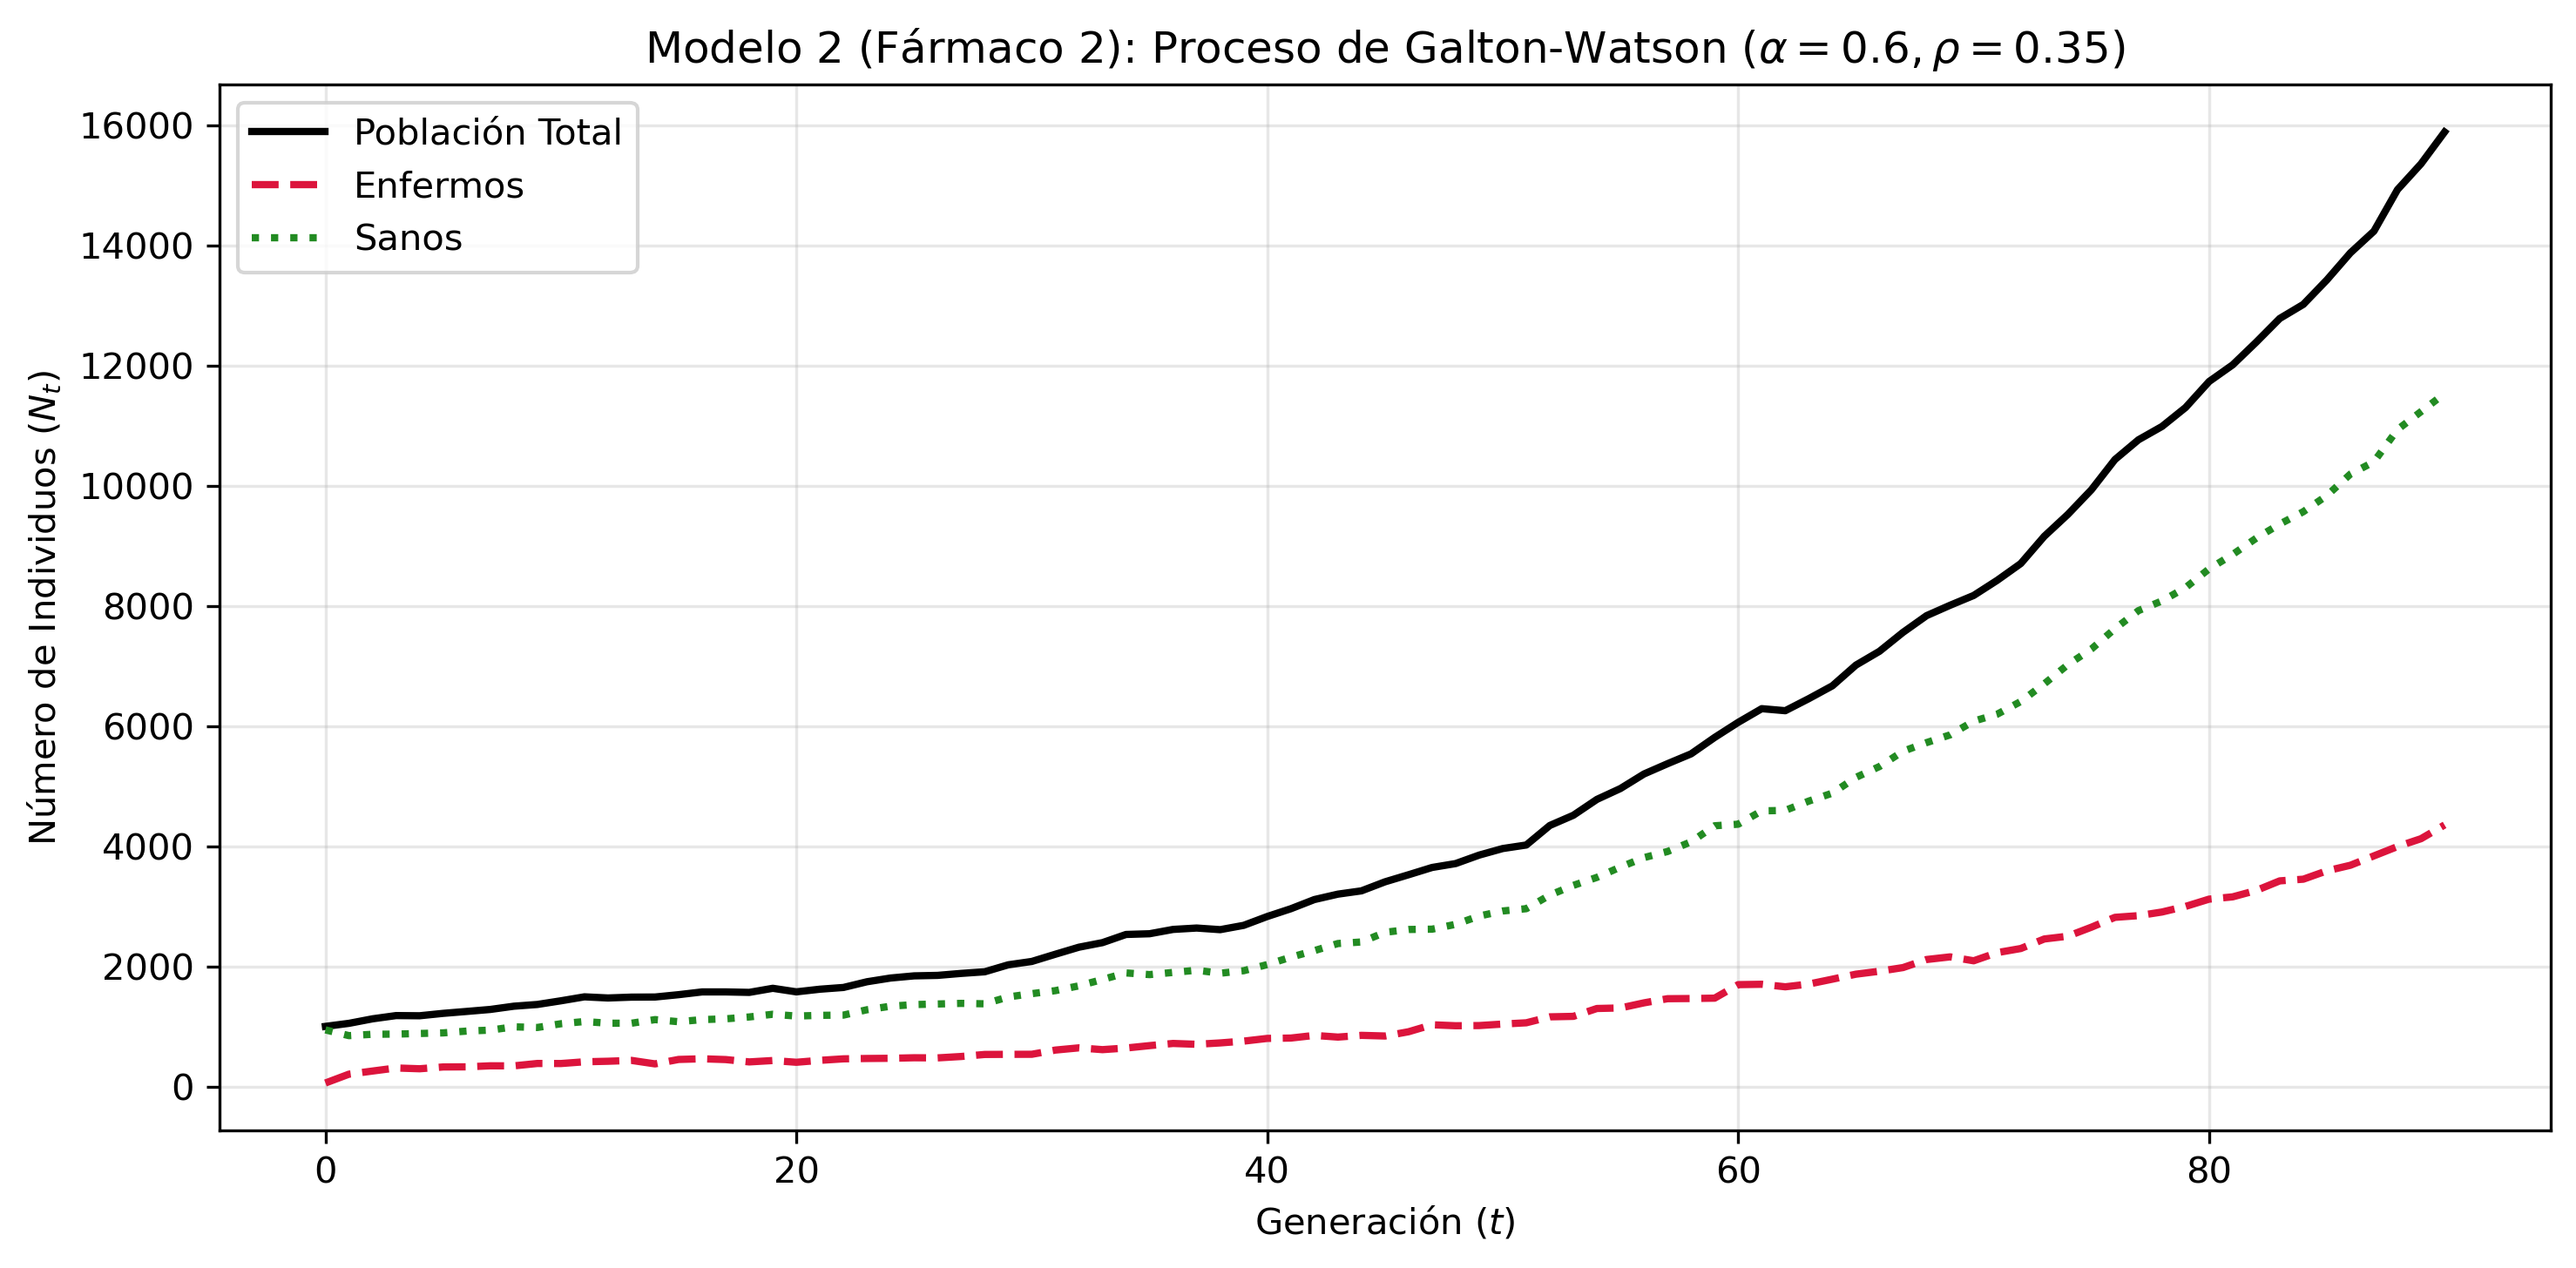
\includegraphics[width=0.85\textwidth]{../imagenes/simulacion_farmaco_2.png}
		\caption{Trayectoria temporal de la población en una única realización con el segundo fármaco ($N_0=1000$, $p_I=0.05$, $\lambda=1.15$, $\alpha=0.6$, $\rho=0.35$). Se observa la evolución de la población total (línea continua negra), sanos (línea punteada verde) y enfermos (línea discontinua roja).}
		\label{fig:simulacion_caso_farmaco_2}
	\end{figure}
	
	La natalidad sigue siendo mayor que la mortalidad, lo que supone el aumento de la población exponencialmente. En cambio, es de interés recalcar que aún existe la enfermedad. Es decir, la población no se extingue, pero la enfermedad tampoco y los casos de enfermos siguen siendo bastante elevados. Esto significa que se ha conseguido disminuir el número de fallecimientos por la enfermedad pero aún se sigue padeciendo. 
	
	En el contexto de este proyecto, que solamente pretende mostrar la evolución y las probabilidades de absorción de la enfermedad, resulta de menor interés la tasa de enfermos siempre y cuando la mortalidad sea pequeña. En cambio, en el contexto real sí que sería bastante importante ya que los individuos afectados podrían tener malestar, lo que podría afectar a la calidad de vida de la población y diferentes aspectos socioeconómicos. 
	
	Al igual que antes, se realiza una simulación de Monte Carlo para disminuir la variabilidad estocástica. 
	
	\begin{figure}[htbp]
		\centering
		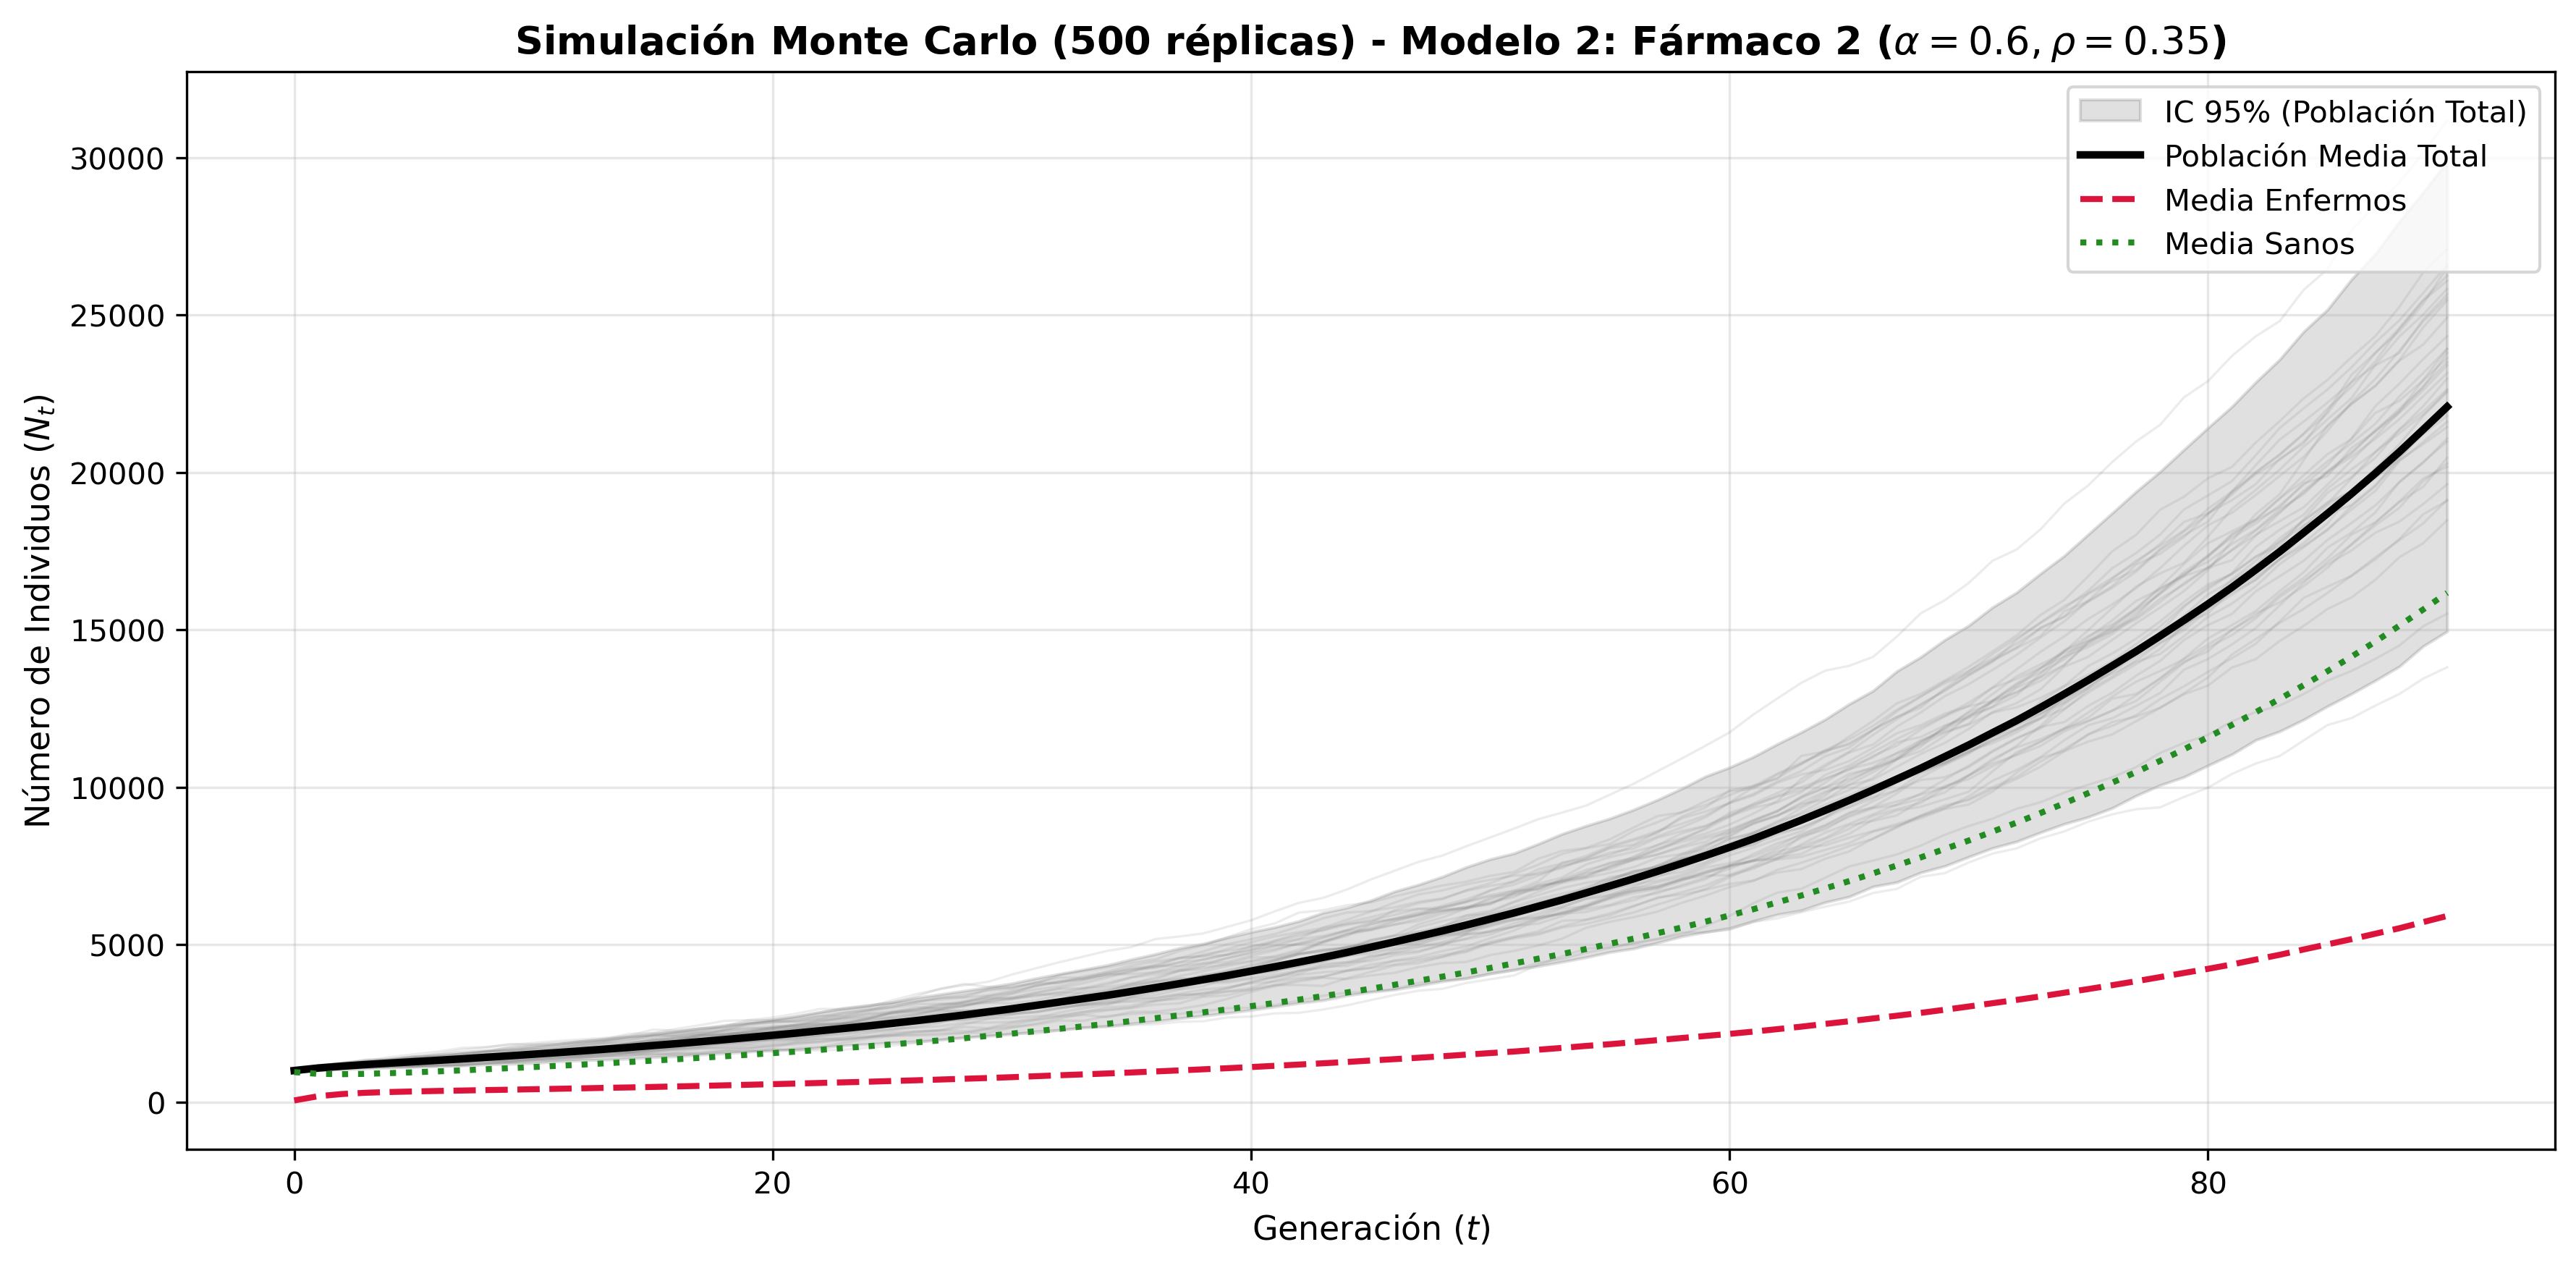
\includegraphics[width=0.85\textwidth]{../imagenes/simulacion_farmaco_2_monte_carlo.png}
		\caption{Trayectoria temporal de la población en múltiples realizaciones con el método de Monte Carlo con el segundo fármaco ($N_0=1000$, $p_I=0.05$, $\lambda=1.15$, $\alpha=0.6$, $\rho=0.35$). Se observa la evolución de la población total (línea continua negra), sanos (línea punteada verde) y enfermos (línea discontinua roja)}
		\label{fig:simulacion_caso_farmaco_2_monte_carlo}
	\end{figure}
	
	Tal y como se expresaba anteriormente, el número de individuos de la población aumenta significativamente a medida que aumentan las generaciones y no se llega a mitigar la enfermedad. 
	
	Al final de las 90 generaciones que nos muestra el horizonte de predicción,  tenemos que aproximadamente 1/4 de la población está enferma y 3/4 se encuentran en estado sano, lo que demuestra experimentalmente que $\mathcal{R}_0^{\text{global}} > 1$ y, como se ha explicado con anterioridad, esto implica la posible no extinción de la población, como es este caso. 
	
	
	\subsection{Resultados de la utilización del tercer fármaco}
	
	Por último, se estudian las consecuencias evolutivas del uso del tercero de los fármacos. Es el que mayor tasa de eficacia y de curación tiene en comparación con el resto de los casos, y se refleja claramente en la simulación de una sola trayectoria. 
	\begin{figure}[htbp]
		\centering
		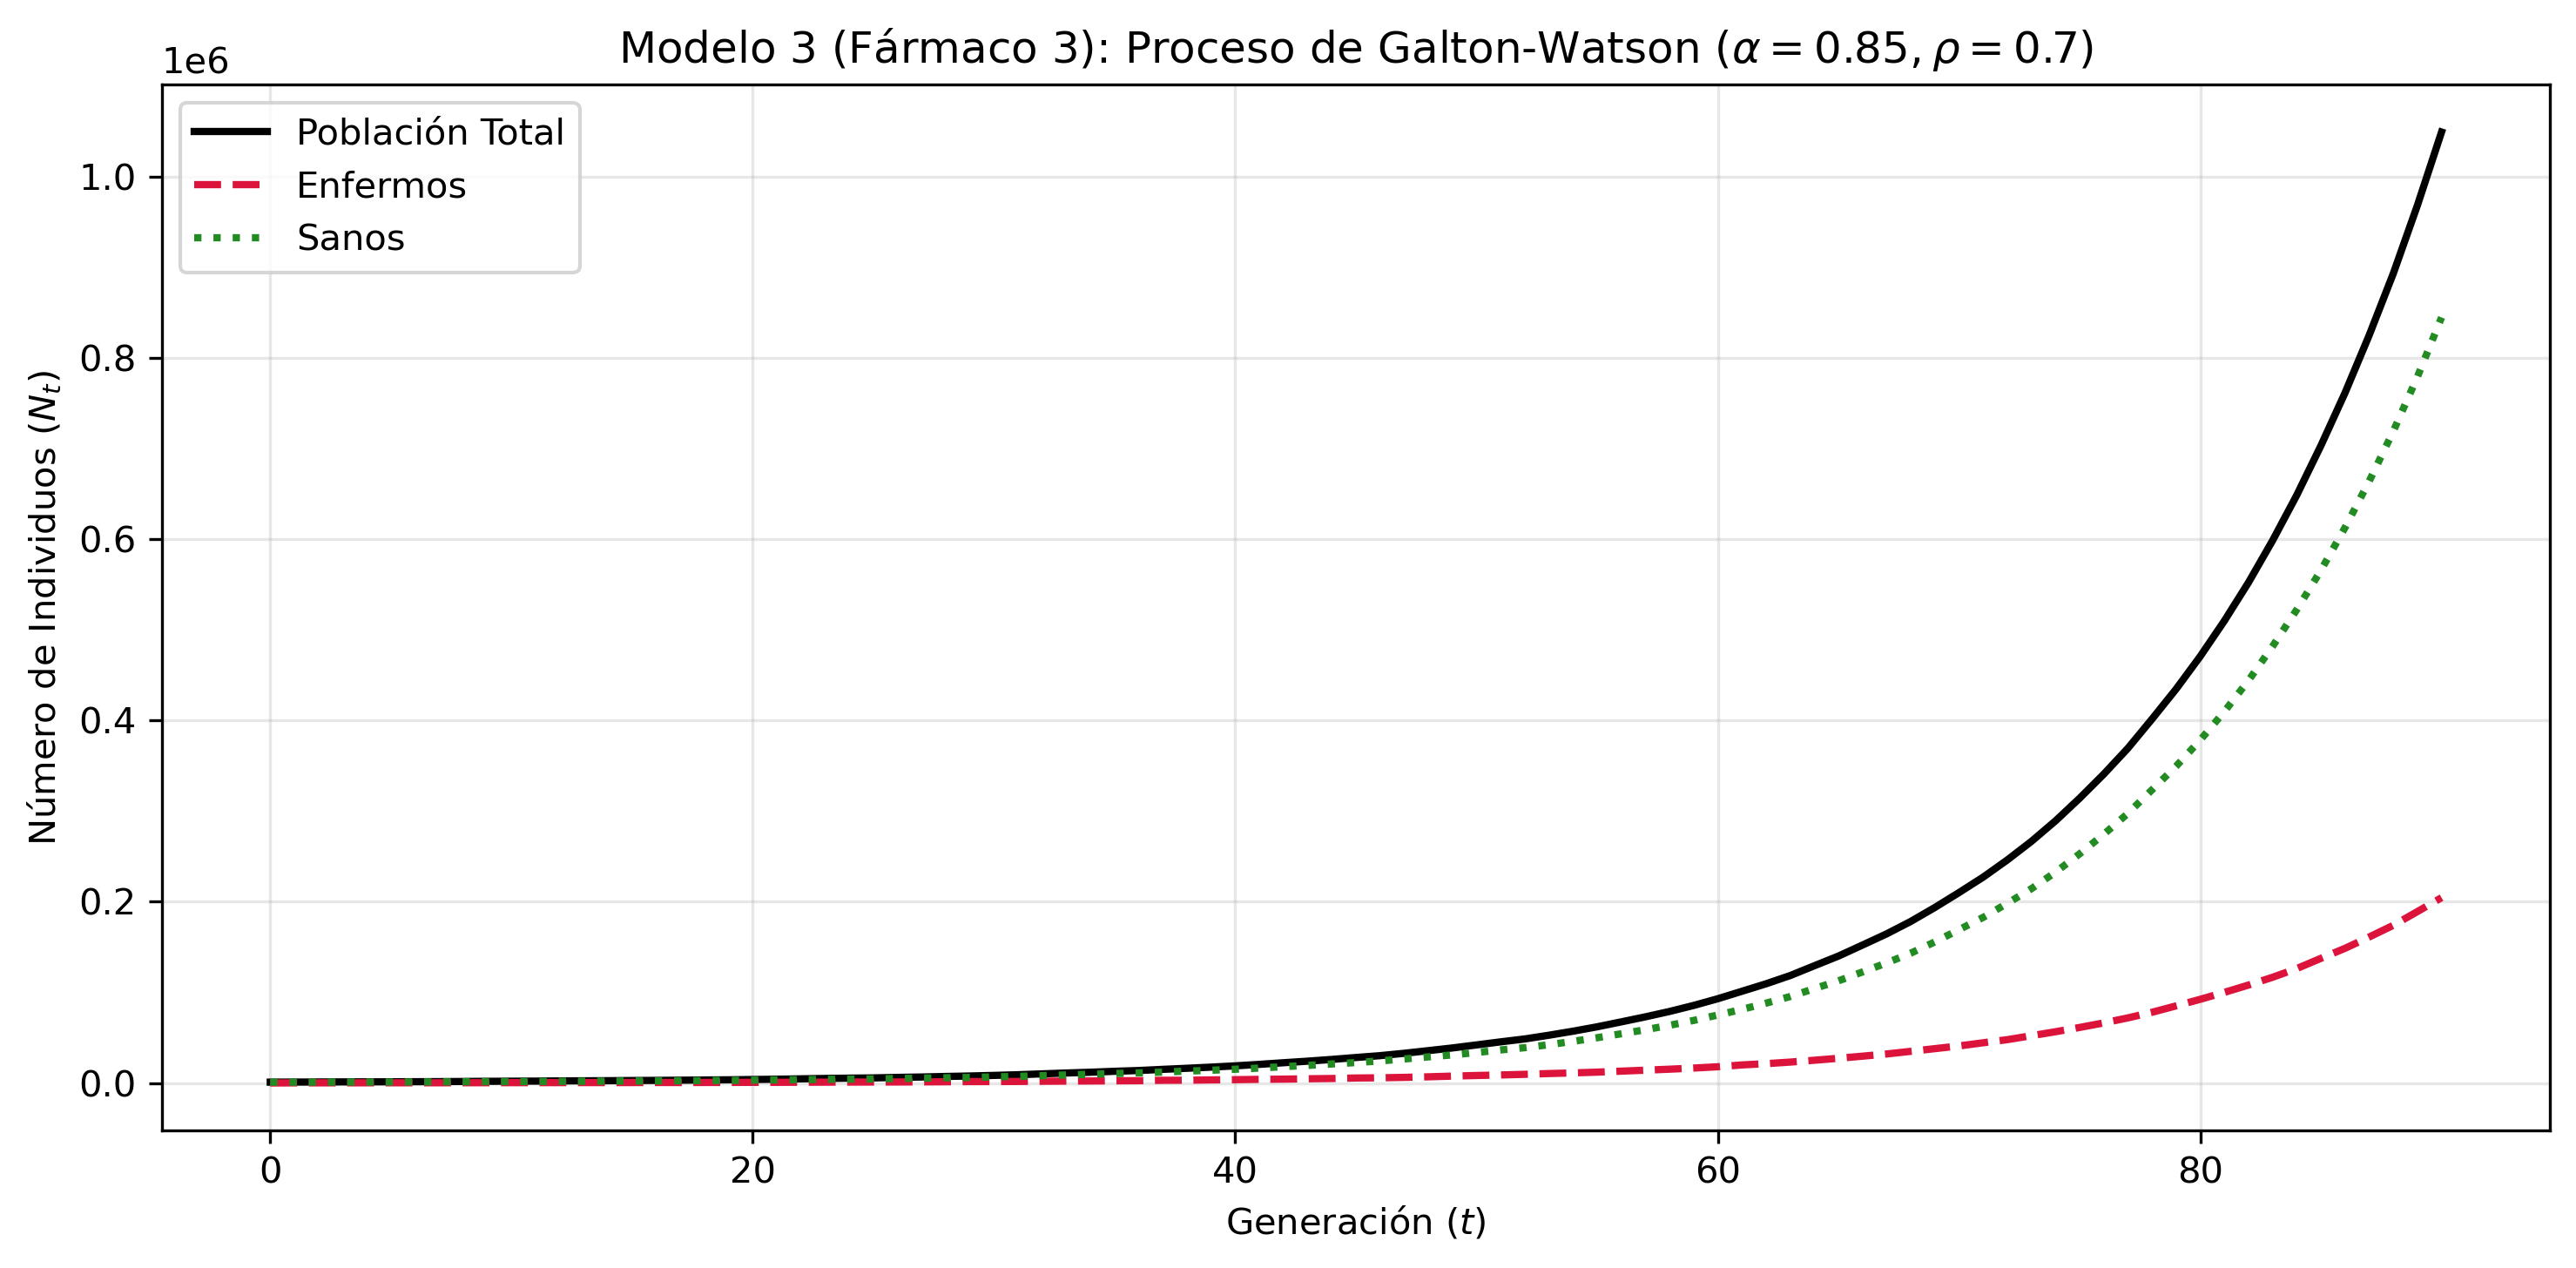
\includegraphics[width=0.85\textwidth]{../imagenes/simulacion_farmaco_3.png}
		\caption{Trayectoria temporal de la población en una única realización con el tercer fármaco ($N_0=1000$, $p_I=0.05$, $\lambda=1.15$, $\alpha=0.85$, $\rho=0.7$). Se observa la evolución de la población total (línea continua negra), sanos (línea punteada verde) y enfermos (línea discontinua roja).}
		\label{fig:simulacion_caso_farmaco_3}
	\end{figure}
	
	Como era de esperar, tampoco se llega a extinguir la población, al igual que con el segundo fármaco. La diferencia principal radica en el número de enfermos en comparación con los individuos sanos. Antes de profundizar más en este tema, se realiza la simulación de Monte Carlo como en el resto de los casos para poder eliminar la variabilidad estocástica que se presenta al estudiar los resultados de una única trayectoria. 
	
	\begin{figure}[htbp]
		\centering
		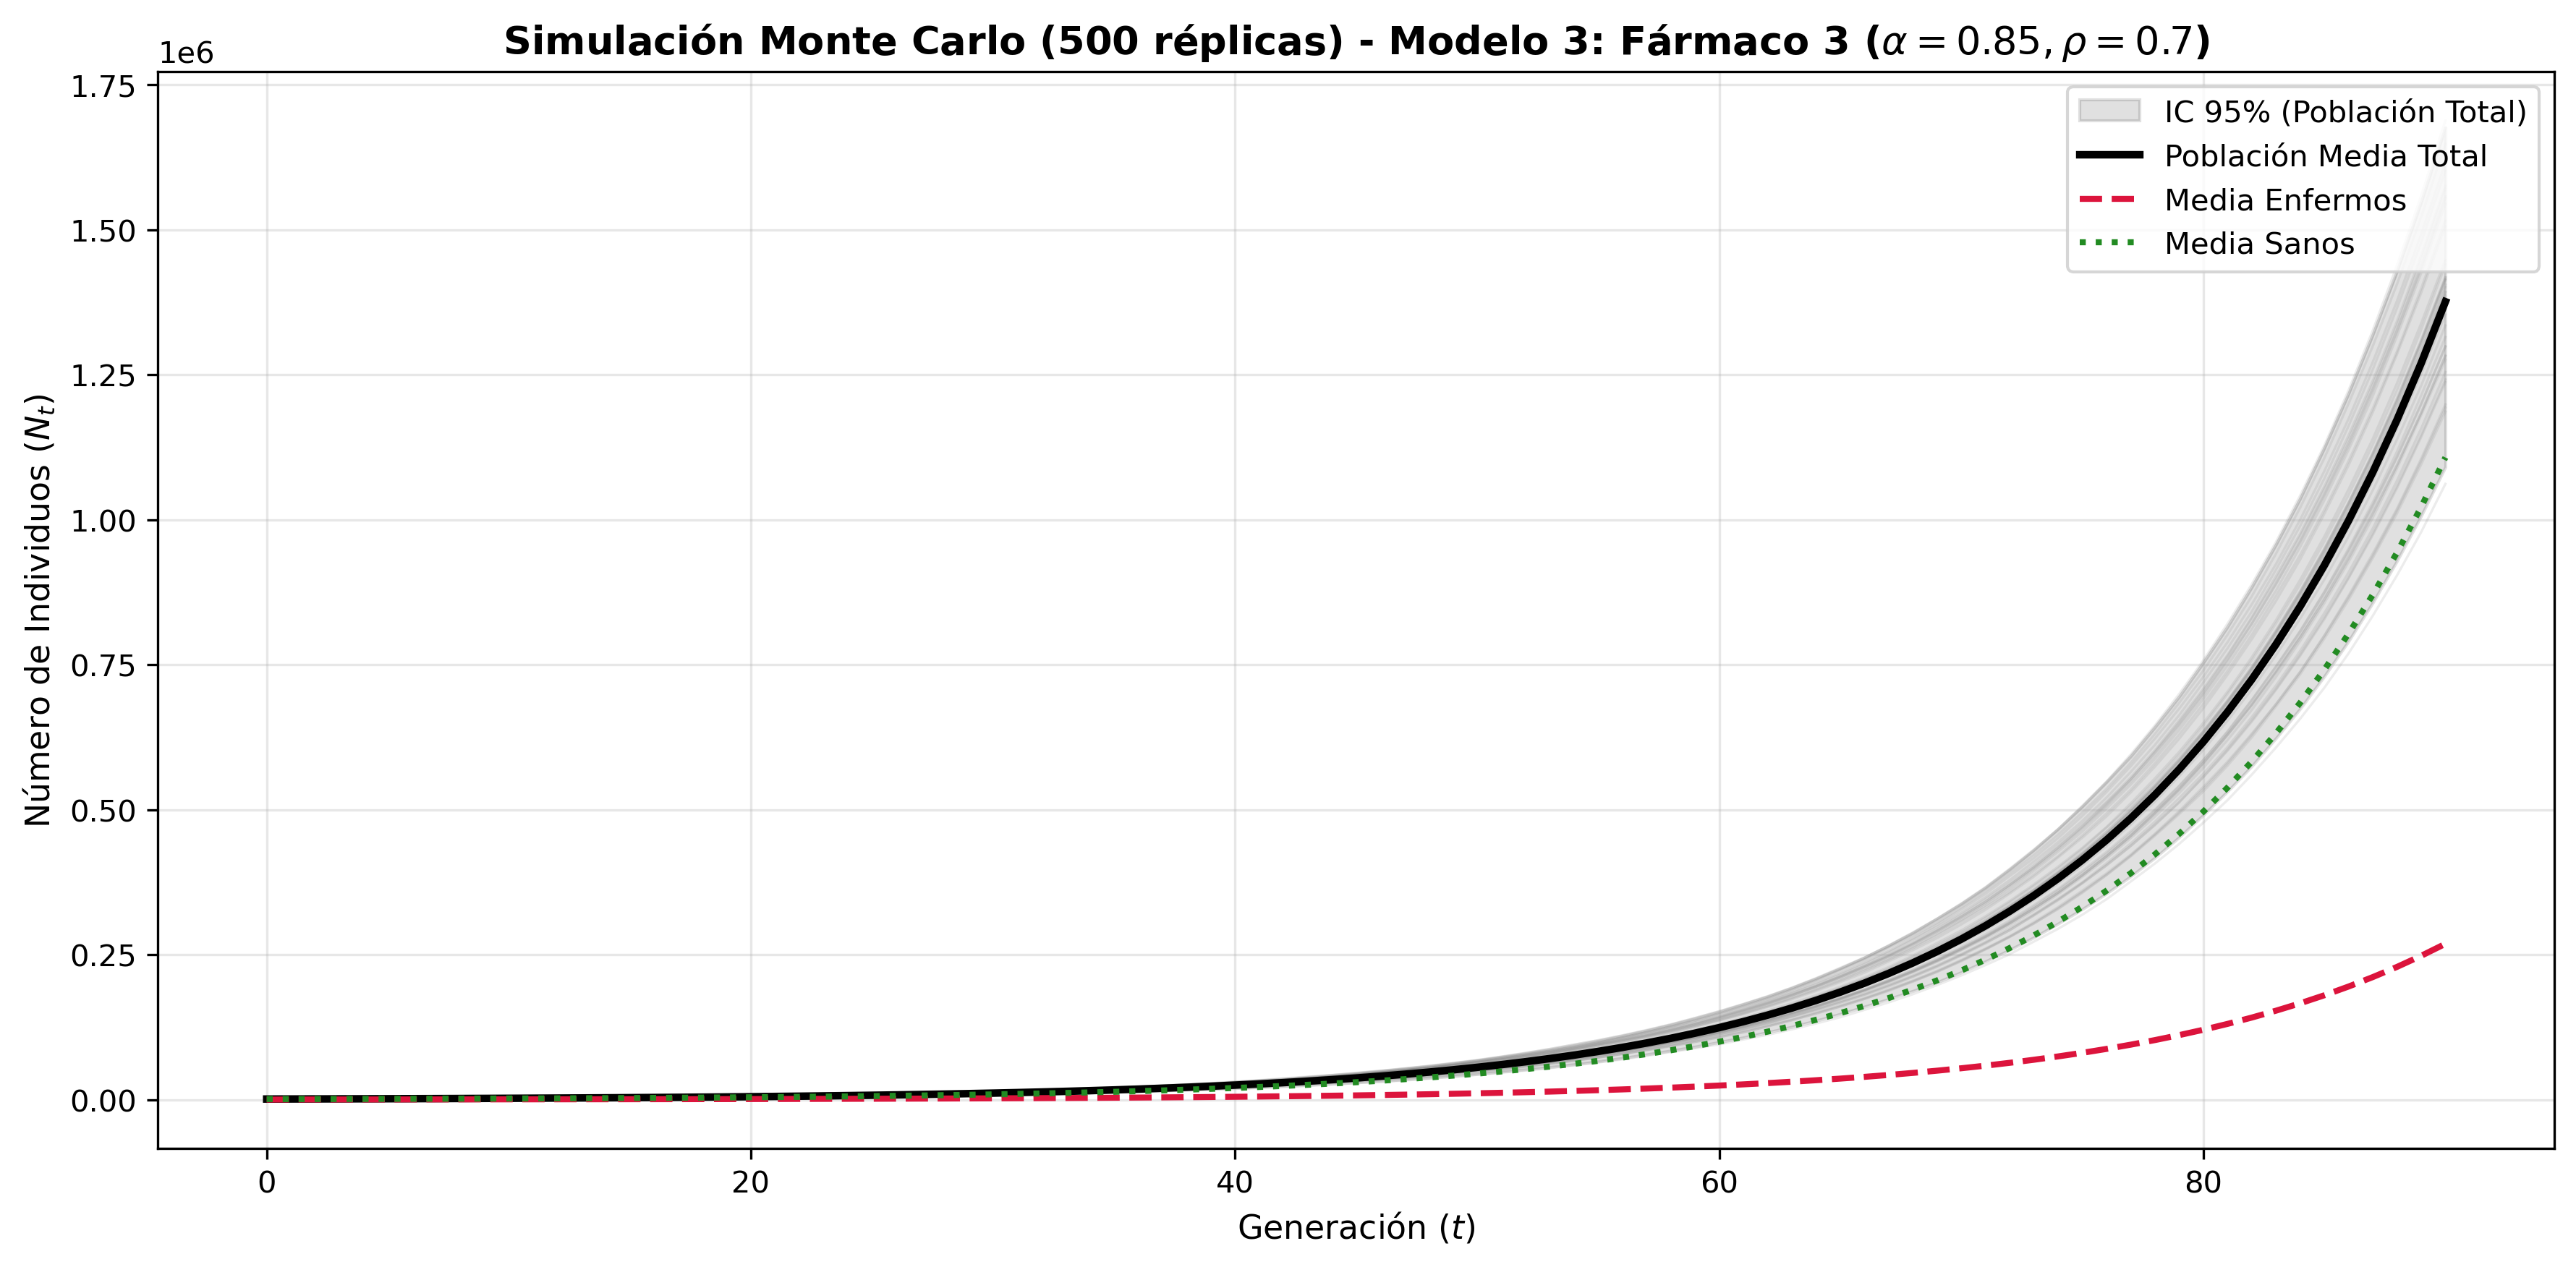
\includegraphics[width=0.85\textwidth]{../imagenes/simulacion_farmaco_3_monte_carlo.png}
		\caption{Trayectoria temporal de la población en múltiples realizaciones con el método de Monte Carlo con el tercer fármaco ($N_0=1000$, $p_I=0.05$, $\lambda=1.15$, $\alpha=0.85$, $\rho=0.7$). Se observa la evolución de la población total (línea continua negra), sanos (línea punteada verde) y enfermos (línea discontinua roja).}
		\label{fig:simulacion_caso_farmaco_3_monte_carlo}
	\end{figure}
	
	Ahora bien, la tasa de sanos aparentemente podría considerarse de 4/5 mientras que la de enfermos 1/5. Como se decía antes, es la principal diferencia que presenta con el otro caso. Además, al disminuir la mortalidad, la población se reproduce significativamente más rápido, lo que implica un mayor número de individuos en la población final. 
	
	Teóricamente, este es el caso que más interés generaría extrapolar a un contexto realista, pero, en la vida real, sería complicado encontrar un medicamento con estas tasas tan elevadas de eficacia y curación. En este proyecto hipotético sirve principalmente para poderlo comparar con el caso anterior. 
	
	
	
	\section{Análisis Comparativo y Discusión de Resultados}
	\label{sec:discusion}
	En el apartado anterior se comentaban las principales diferencias entre el uso de diferentes fármacos en comparación con el Caso Base y entre ellos. En este apartado se añaden algunas conclusiones sobre dichas comparaciones y una tabla que permite sintetizar de manera visual lo dicho anteriormente. 
	
	
	Para integrar los resultados analíticos de la teoría de ramificación con las estimaciones empíricas obtenidas mediante Monte Carlo ($M=500$), la Tabla~\ref{tab:comparativa_global_final} resume el comportamiento completo del sistema en los cuatro escenarios analizados.
	
	\begin{table}[htbp]
		\caption{Comparativa global entre predicciones teóricas ($\mathcal{R}_0^{\text{global}}$, $\eta_{\text{total}}$) y resultados empíricos de Monte Carlo ($M=500$, $t_{\max}=90$) para el Caso Base y los tres modelos farmacológicos.}
		\label{tab:comparativa_global_final}
		\centering
		\begin{tabular}{lcccccc}
			\hline
			\textbf{Escenario} & $(\alpha, \rho)$ & $\mathcal{R}_0^{\text{global}}$ & $\eta_{\text{total}}$ \textbf{(Teo.)} & \textbf{Extinción ($t \le 90$)} & $\mathbb{E}[N_{90}]$ \textbf{(Media)} & \textbf{Ratio Sanos / Enf.} \\
			\hline
			Caso Base & $(0.00, 0.00)$ & $0.9362$ & $1.0000$ & $71.00\%$ & $\approx 12$ & $70.5\% \, / \, 29.5\%$ \\
			Fármaco 1 & $(0.30, 0.10)$ & $0.9655$ & $1.0000$ & $6.40\%$ & $\approx 52$ & $70.6\% \, / \, 29.4\%$ \\
			Fármaco 2 & $(0.60, 0.35)$ & $1.0340$ & $\approx 0$ & $0.00\%$ & $22\,102$ & $73.2\% \, / \, 26.8\%$ \\
			Fármaco 3 & $(0.85, 0.70)$ & $1.0835$ & $\approx 0$ & $0.00\%$ & $1\,384\,281$ & $80.5\% \, / \, 19.5\%$ \\
			\hline
		\end{tabular}
	\end{table}
	
	\section{Análisis de la complejidad computacional}
	Se presenta un problema crítico cuando se tratan de ejecutar las simulaciones de Monte Carlo cuando la población no converge a la absorción. Ocurre debido a que el número de individuos de cada generación aumenta exponencialmente y la complejidad asintótica promedio pasa a ser demasiado elevada. Esto supone un tiempo de cómputo demasiado largo. 
	
	Para superar este cuello de botella sin alterar la exactitud estocástica del modelo, se aplicó una \textit{reducción analítica mediante propiedades de aditividad de distribuciones} (vectorización por compartimentos):
	\begin{enumerate}
		\item \textbf{Supervivencia y curación (Propiedad Binomial):} Dado que los individuos de un mismo estado evolucionan de forma independiente e idénticamente distribuida (i.i.d.), la suma de $S_t$ ensayos de Bernoulli independientes con probabilidad de supervivencia $(1 - m_0)$ sigue exactamente una distribución $\text{Binomial}(S_t, 1 - m_0)$.
		\item \textbf{Reproducción agregada (Propiedad reproductiva de Poisson):} Por la estabilidad bajo suma de la distribución de Poisson, la descendencia total generada por $S_{t,\text{rep}}$ progenitores independientes con tasa individual $\lambda$ equivale exactamente a una única realización de $\text{Poisson}(S_{t,\text{rep}} \cdot \lambda)$.
	\end{enumerate}
	
	De esta forma se consigue que la complejidad asintótica disminuya de varias horas a tan solo unos segundos. 
	
	\section{Conclusiones y Trabajos Futuros}
	\label{sec:conclusiones}
	Se obtienen diferentes conclusiones a lo largo del proyecto. 
	
	\subsection{Amenaza de la enfermedad respecto a la población}
	Como se ha visto anteriormente en el Caso Base, la enfermedad supone una gran amenaza en la población debido a la probabilidad de extinción irreversible $\eta = 1$. 
	
	Por este mismo motivo es que se proponen tres soluciones, aunque la primera únicamente serviría para posponer la extinción de manera temporal. 
	
	\subsection{Tres soluciones propuestas}
	Como ya se ha comentado, la primera no impediría la extinción, pero podría resultar útil aplicarla mientras se busca otra más eficaz y con mayor tasa curativa. 
	
	Por otra parte, no se debe buscar un fármaco que simplemente mantenga a la población viva, sino que es relevante que la mantenga sana. En este proyecto no se valoran las consecuencias de la enfermedad más allá de la muerte, pero debería estudiarse. 
	
	La tercera es la mejor solución entre las tres. Este medicamento es el que maximiza la población sana, la reproducción y evita la extinción de la población. Aun así, tampoco es capaz de erradicar la enfermedad. 
	
	\subsection{Realidad}
	Se ha tratado de realizar el proyecto hipotético dentro de unos marcos realistas, pero, de todas formas, sigue sin ser adecuado a la realidad. Se tendría que tener en cuenta mucho más parámetros y situaciones para considerarlo completo. 
	
	También se ha tratado de llevar las conclusiones más allá de lo que simplemente dicen los datos, sino lo que realmente significaría en un contexto clínico real. 
	
	El objetivo principal del proyecto es simplemente ver como evolucionaría la reproducción, el número de individuos en la población y la tasa de enfermos en la población, enfocándolo principalmente a la extinción o supervivencia de la población ante la enfermedad. 
	
	Se ha tratado de estudiar tanto de forma teórica como de forma experimental con simulaciones de Monte Carlo durante todo el proyecto. 
	
	\subsection{Diferentes propuestas a futuro}
	Al proyecto le faltarían muchas situaciones y parámetros diferentes para ser más cercanos a la realidad, en esta sección se presentan unos cuantos aspectos interesantes que podrían ser estudiados en un futuro. 
	
	\subsubsection{Tiempo de obtención del fármaco}
	Desde el primer momento se supone una población finita con un cierto porcentaje de enfermos. En ese mismo momento se empiezan a aplicar los diferentes fármacos. 
	
	En cambio, en un contexto más realista, desde que se comienzan a investigar los casos, se estudia la enfermedad y se encuentra una o varias alternativas de medicamentos que puedan resultar útiles tarda un tiempo significativo. Con esto se quiere decir que podría ocurrir que la enfermedad se propague demasiado rápido y cuando se quiera aplicar el fármaco sea ya irremediable el estado de absorción. También podría darse la situación en la que no se encuentra ningún fármaco que consiga erradicar la enfermedad. 
	
	Sea como sea, se debería tener en cuenta el tiempo medio que podría requerir encontrar una solución factible para el problema y no asumir que ya se tiene. 
	
	\subsubsection{Consecuencias del estado enfermo}
	Se ha omitido el estudio de posibles consecuencias que podría suponer el estado enfermo a la hora de la evolución de la población. Podría ocurrir que entre los principales síntomas de la enfermedad se encuentren problemas de fertilidad, que supondría una disminución drástica de la natalidad aunque los individuos enfermos sobrevivan. 
	
	También podría afectar a la calidad de vida de la población y otros factores socioeconómicos de la población. Todo esto se ha omitido durante el proyecto ya que, al tratarse de una enfermedad hipotética, no se han establecido síntomas. 
	
	\subsubsection{Factores socioeconómicos y culturales}
	Se tiene en cuenta que todos los individuos se reproducen de igual forma y tienen los mismos medios para obtener los fármacos. Esto no es realista. En función de la cultura, por ejemplo, se puede tener más acceso a sanidad o fármacos. También varía el número de hijos y la esperanza media de reproducción según países y cultura. Otras situaciones que podrían ocurrir en la realidad sería que se desarrolle una medicación apta para el desarrollo de la población, pero no llegue a todos los países o culturas. 
	
	\subsubsection{Resistencias farmacológicas}
	No se tiene en cuenta el tiempo de eficacia que tiene el fármaco, o si quizás con el paso del tiempo las generaciones se inmunizan del fármaco y vuelve a aumentar su probabilidad de padecer la enfermedad o fallecer. 
	
	
	
\end{document}